\documentclass[11pt,]{article}
\usepackage[left=1in,top=1in,right=1in,bottom=1in]{geometry}
\newcommand*{\authorfont}{\fontfamily{phv}\selectfont}
\usepackage[]{mathpazo}


  \usepackage[T1]{fontenc}
  \usepackage[utf8]{inputenc}



\usepackage{abstract}
\renewcommand{\abstractname}{}    % clear the title
\renewcommand{\absnamepos}{empty} % originally center

\renewenvironment{abstract}
 {{%
    \setlength{\leftmargin}{0mm}
    \setlength{\rightmargin}{\leftmargin}%
  }%
  \relax}
 {\endlist}

\makeatletter
\def\@maketitle{%
  \newpage
%  \null
%  \vskip 2em%
%  \begin{center}%
  \let \footnote \thanks
    {\fontsize{18}{20}\selectfont\raggedright  \setlength{\parindent}{0pt} \@title \par}%
}
%\fi
\makeatother




\setcounter{secnumdepth}{0}

\usepackage{color}
\usepackage{fancyvrb}
\newcommand{\VerbBar}{|}
\newcommand{\VERB}{\Verb[commandchars=\\\{\}]}
\DefineVerbatimEnvironment{Highlighting}{Verbatim}{commandchars=\\\{\}}
% Add ',fontsize=\small' for more characters per line
\usepackage{framed}
\definecolor{shadecolor}{RGB}{248,248,248}
\newenvironment{Shaded}{\begin{snugshade}}{\end{snugshade}}
\newcommand{\KeywordTok}[1]{\textcolor[rgb]{0.13,0.29,0.53}{\textbf{{#1}}}}
\newcommand{\DataTypeTok}[1]{\textcolor[rgb]{0.13,0.29,0.53}{{#1}}}
\newcommand{\DecValTok}[1]{\textcolor[rgb]{0.00,0.00,0.81}{{#1}}}
\newcommand{\BaseNTok}[1]{\textcolor[rgb]{0.00,0.00,0.81}{{#1}}}
\newcommand{\FloatTok}[1]{\textcolor[rgb]{0.00,0.00,0.81}{{#1}}}
\newcommand{\ConstantTok}[1]{\textcolor[rgb]{0.00,0.00,0.00}{{#1}}}
\newcommand{\CharTok}[1]{\textcolor[rgb]{0.31,0.60,0.02}{{#1}}}
\newcommand{\SpecialCharTok}[1]{\textcolor[rgb]{0.00,0.00,0.00}{{#1}}}
\newcommand{\StringTok}[1]{\textcolor[rgb]{0.31,0.60,0.02}{{#1}}}
\newcommand{\VerbatimStringTok}[1]{\textcolor[rgb]{0.31,0.60,0.02}{{#1}}}
\newcommand{\SpecialStringTok}[1]{\textcolor[rgb]{0.31,0.60,0.02}{{#1}}}
\newcommand{\ImportTok}[1]{{#1}}
\newcommand{\CommentTok}[1]{\textcolor[rgb]{0.56,0.35,0.01}{\textit{{#1}}}}
\newcommand{\DocumentationTok}[1]{\textcolor[rgb]{0.56,0.35,0.01}{\textbf{\textit{{#1}}}}}
\newcommand{\AnnotationTok}[1]{\textcolor[rgb]{0.56,0.35,0.01}{\textbf{\textit{{#1}}}}}
\newcommand{\CommentVarTok}[1]{\textcolor[rgb]{0.56,0.35,0.01}{\textbf{\textit{{#1}}}}}
\newcommand{\OtherTok}[1]{\textcolor[rgb]{0.56,0.35,0.01}{{#1}}}
\newcommand{\FunctionTok}[1]{\textcolor[rgb]{0.00,0.00,0.00}{{#1}}}
\newcommand{\VariableTok}[1]{\textcolor[rgb]{0.00,0.00,0.00}{{#1}}}
\newcommand{\ControlFlowTok}[1]{\textcolor[rgb]{0.13,0.29,0.53}{\textbf{{#1}}}}
\newcommand{\OperatorTok}[1]{\textcolor[rgb]{0.81,0.36,0.00}{\textbf{{#1}}}}
\newcommand{\BuiltInTok}[1]{{#1}}
\newcommand{\ExtensionTok}[1]{{#1}}
\newcommand{\PreprocessorTok}[1]{\textcolor[rgb]{0.56,0.35,0.01}{\textit{{#1}}}}
\newcommand{\AttributeTok}[1]{\textcolor[rgb]{0.77,0.63,0.00}{{#1}}}
\newcommand{\RegionMarkerTok}[1]{{#1}}
\newcommand{\InformationTok}[1]{\textcolor[rgb]{0.56,0.35,0.01}{\textbf{\textit{{#1}}}}}
\newcommand{\WarningTok}[1]{\textcolor[rgb]{0.56,0.35,0.01}{\textbf{\textit{{#1}}}}}
\newcommand{\AlertTok}[1]{\textcolor[rgb]{0.94,0.16,0.16}{{#1}}}
\newcommand{\ErrorTok}[1]{\textcolor[rgb]{0.64,0.00,0.00}{\textbf{{#1}}}}
\newcommand{\NormalTok}[1]{{#1}}

\usepackage{graphicx}
% We will generate all images so they have a width \maxwidth. This means
% that they will get their normal width if they fit onto the page, but
% are scaled down if they would overflow the margins.
\makeatletter
\def\maxwidth{\ifdim\Gin@nat@width>\linewidth\linewidth
\else\Gin@nat@width\fi}
\makeatother
\let\Oldincludegraphics\includegraphics
\renewcommand{\includegraphics}[1]{\Oldincludegraphics[width=\maxwidth]{#1}}

\title{Cuvier's beaked whale habitat models  }



\author{\Large Kaitlin E. Frasier\vspace{0.05in} \newline\normalsize\emph{SIO UCSD}   \and \Large Lance P. Garrison\vspace{0.05in} \newline\normalsize\emph{NOAA SEFSC}   \and \Large Melissa S. Soldevilla\vspace{0.05in} \newline\normalsize\emph{NOAA SEFSC}   \and \Large Sean M. Wiggins\vspace{0.05in} \newline\normalsize\emph{SIO UCSD}   \and \Large John A. Hildebrand\vspace{0.05in} \newline\normalsize\emph{SIO UCSD}  }


\date{}

\usepackage{titlesec}

\titleformat*{\section}{\normalsize\bfseries}
\titleformat*{\subsection}{\normalsize\itshape}
\titleformat*{\subsubsection}{\normalsize\itshape}
\titleformat*{\paragraph}{\normalsize\itshape}
\titleformat*{\subparagraph}{\normalsize\itshape}


\usepackage{natbib}
\bibliographystyle{apsr}
\usepackage[strings]{underscore} % protect underscores in most circumstances



\newtheorem{hypothesis}{Hypothesis}
\usepackage{setspace}

\makeatletter
\@ifpackageloaded{hyperref}{}{%
\ifxetex
  \PassOptionsToPackage{hyphens}{url}\usepackage[setpagesize=false, % page size defined by xetex
              unicode=false, % unicode breaks when used with xetex
              xetex]{hyperref}
\else
  \PassOptionsToPackage{hyphens}{url}\usepackage[unicode=true]{hyperref}
\fi
}

\@ifpackageloaded{color}{
    \PassOptionsToPackage{usenames,dvipsnames}{color}
}{%
    \usepackage[usenames,dvipsnames]{color}
}
\makeatother
\hypersetup{breaklinks=true,
            bookmarks=true,
            pdfauthor={Kaitlin E. Frasier (SIO UCSD) and Lance P. Garrison (NOAA SEFSC) and Melissa S. Soldevilla (NOAA SEFSC) and Sean M. Wiggins (SIO UCSD) and John A. Hildebrand (SIO UCSD)},
             pdfkeywords = {},  
            pdftitle={Cuvier's beaked whale habitat models},
            colorlinks=true,
            citecolor=blue,
            urlcolor=blue,
            linkcolor=magenta,
            pdfborder={0 0 0}}
\urlstyle{same}  % don't use monospace font for urls



% add tightlist ----------
\providecommand{\tightlist}{%
\setlength{\itemsep}{0pt}\setlength{\parskip}{0pt}}

\begin{document}
	
% \pagenumbering{arabic}% resets `page` counter to 1 
%
% \maketitle

{% \usefont{T1}{pnc}{m}{n}
\setlength{\parindent}{0pt}
\thispagestyle{plain}
{\fontsize{18}{20}\selectfont\raggedright 
\maketitle  % title \par  

}

{
   \vskip 13.5pt\relax \normalsize\fontsize{11}{12} 
\textbf{\authorfont Kaitlin E. Frasier} \hskip 15pt \emph{\small SIO UCSD}   \par \textbf{\authorfont Lance P. Garrison} \hskip 15pt \emph{\small NOAA SEFSC}   \par \textbf{\authorfont Melissa S. Soldevilla} \hskip 15pt \emph{\small NOAA SEFSC}   \par \textbf{\authorfont Sean M. Wiggins} \hskip 15pt \emph{\small SIO UCSD}   \par \textbf{\authorfont John A. Hildebrand} \hskip 15pt \emph{\small SIO UCSD}   

}

}






\vskip 6.5pt


\noindent  \begin{Shaded}
\begin{Highlighting}[]
\KeywordTok{library}\NormalTok{(mgcv)}
\KeywordTok{library}\NormalTok{(MASS)}
\KeywordTok{library}\NormalTok{(rgdal)}
\KeywordTok{library}\NormalTok{(raster)}
\KeywordTok{library}\NormalTok{(ggplot2)}
\KeywordTok{library}\NormalTok{(rgeos)}
\KeywordTok{library}\NormalTok{(mapview)}
\KeywordTok{library}\NormalTok{(leaflet)}
\KeywordTok{library}\NormalTok{(psych)}
\KeywordTok{library}\NormalTok{(broom)}
\KeywordTok{library}\NormalTok{(plotrix)}
\KeywordTok{library}\NormalTok{(magrittr)}
\KeywordTok{library}\NormalTok{(colorRamps)}
\KeywordTok{library}\NormalTok{(lubridate)}
\KeywordTok{library}\NormalTok{(HabitatProject)}
\KeywordTok{library}\NormalTok{(lmtest)}
\KeywordTok{source}\NormalTok{(}\StringTok{'E:/NASData/AcoustoVisualDE/AcoustoVisualDE/HabitatProject/R/multiplot.R'}\NormalTok{)}
\KeywordTok{options}\NormalTok{(}\DataTypeTok{stringsAsFactors =} \OtherTok{FALSE}\NormalTok{)}
\CommentTok{# load some preferences}
\KeywordTok{load}\NormalTok{(}\StringTok{'E:/NASData/ModelData/Zc/setup_info_Zc.Rdata'}\NormalTok{)}
\KeywordTok{load}\NormalTok{(}\StringTok{'E:/NASData/ModelData/Zc/ZcMergedData.Rdata'}\NormalTok{)}
\NormalTok{outDir <-}\StringTok{ }\KeywordTok{file.path}\NormalTok{(}\StringTok{'E:/NASData/ModelData'}\NormalTok{,SP,}\StringTok{'/'}\NormalTok{)}
\end{Highlighting}
\end{Shaded}

\section{I. Exploratory analysis}\label{i.-exploratory-analysis}

\subsection{Data Inputs}\label{data-inputs}

The visual data goes back to 1992, but as shown in the figure below,
many predictor variables are only available starting in 2003, therefore
earlier visual data is currently excluded from further analyses.

Note: Future work could use monthly climatologies (averages) so that
older sightings data could be used. Some dynamic drivers like eddy and
front locations would not be able to be considered using that approach.

\begin{Shaded}
\begin{Highlighting}[]
\NormalTok{covarList<-}\KeywordTok{names}\NormalTok{(mergedSegments[}\KeywordTok{c}\NormalTok{(}\DecValTok{2}\NormalTok{,}\DecValTok{5}\NormalTok{:}\KeywordTok{length}\NormalTok{(mergedSegments))])}

\NormalTok{percFilled <-}\StringTok{ }\KeywordTok{plot.missingdata}\NormalTok{(mergedSegments,covarList,}\KeywordTok{paste0}\NormalTok{(outDir,}\StringTok{'AcousticAndVisual_'}\NormalTok{,SP)) }
\NormalTok{percFilled <-}\StringTok{ }\KeywordTok{plot.missingdata}\NormalTok{(AcOnlySegments,covarList,}\KeywordTok{paste0}\NormalTok{(outDir,}\StringTok{'AcousticOnly_'}\NormalTok{,SP)) }
\NormalTok{percFilled <-}\StringTok{ }\KeywordTok{plot.missingdata}\NormalTok{(VisOnlySegments,covarList,}\KeywordTok{paste0}\NormalTok{(outDir,}\StringTok{'VisualOnly_'}\NormalTok{,SP)) }
\end{Highlighting}
\end{Shaded}

\includegraphics{E:/NASData/ModelData/Zc/AcousticOnly_Zc_missingData.png}

\subsubsection{Testing and Training
Sets}\label{testing-and-training-sets}

The data are split into training and testing sets. In this case, data
from 2009 and 2013 are used for testing. Only observations post-2003 are
used for modeling due to covariate limitations.

\begin{Shaded}
\begin{Highlighting}[]
\CommentTok{# If you decide from the missing data plots that you want to restrict years going forward:}
\NormalTok{yearListIdx =}\StringTok{ }\KeywordTok{as.numeric}\NormalTok{(}\KeywordTok{format}\NormalTok{(mergedSegments$date,}\StringTok{"%Y"}\NormalTok{))}
\NormalTok{yearListIdx_AcOnly =}\StringTok{ }\KeywordTok{as.numeric}\NormalTok{(}\KeywordTok{format}\NormalTok{(AcOnlySegments$date,}\StringTok{"%Y"}\NormalTok{))}
\NormalTok{yearListIdx_VisOnly =}\StringTok{ }\KeywordTok{as.numeric}\NormalTok{(}\KeywordTok{format}\NormalTok{(VisOnlySegments$date,}\StringTok{"%Y"}\NormalTok{))}

\NormalTok{keepDates.train <-}\StringTok{ }\KeywordTok{which}\NormalTok{(yearListIdx !=}\StringTok{ }\DecValTok{2009} \NormalTok{&}\StringTok{ }\NormalTok{yearListIdx >=}\StringTok{ }\DecValTok{2003} \NormalTok{&}\StringTok{ }\NormalTok{yearListIdx <=}\StringTok{ }\DecValTok{2012}\NormalTok{)}
\NormalTok{keepDates.test <-}\StringTok{ }\KeywordTok{which}\NormalTok{(yearListIdx ==}\StringTok{ }\DecValTok{2009} \NormalTok{|}\StringTok{ }\NormalTok{yearListIdx ==}\StringTok{ }\DecValTok{2013}\NormalTok{)}
\NormalTok{keepDates_AcOnly.train <-}\StringTok{ }\KeywordTok{which}\NormalTok{(yearListIdx_AcOnly !=}\StringTok{ }\DecValTok{2009} \NormalTok{&}\StringTok{ }\NormalTok{yearListIdx_AcOnly >=}\StringTok{ }\DecValTok{2003} \NormalTok{&}\StringTok{ }\NormalTok{yearListIdx_AcOnly <=}\StringTok{ }\DecValTok{2012}\NormalTok{)}
\NormalTok{keepDates_AcOnly.test <-}\StringTok{ }\KeywordTok{which}\NormalTok{(yearListIdx_AcOnly ==}\StringTok{ }\DecValTok{2009} \NormalTok{|}\StringTok{ }\NormalTok{yearListIdx_AcOnly ==}\StringTok{ }\DecValTok{2013}\NormalTok{)}
\NormalTok{keepDatesVisOnly.train <-}\StringTok{ }\KeywordTok{which}\NormalTok{(yearListIdx_VisOnly !=}\StringTok{ }\DecValTok{2009} \NormalTok{&}\StringTok{ }\NormalTok{yearListIdx_VisOnly >=}\StringTok{ }\DecValTok{2003}\NormalTok{)}
\NormalTok{keepDatesVisOnly.test <-}\StringTok{ }\KeywordTok{which}\NormalTok{(yearListIdx_VisOnly ==}\StringTok{ }\DecValTok{2009}\NormalTok{)}

\NormalTok{mergedTrain.set<-}\StringTok{ }\NormalTok{mergedSegments[keepDates.train,]}
\NormalTok{Train_AcOnly.set <-}\StringTok{ }\NormalTok{AcOnlySegments[keepDates_AcOnly.train,]}
\NormalTok{Train_VisOnly.set<-}\StringTok{ }\NormalTok{VisOnlySegments[keepDatesVisOnly.train,]}

\NormalTok{mergedTest.set<-}\StringTok{ }\NormalTok{mergedSegments[keepDates.test,]}
\NormalTok{Test_AcOnly.set<-}\StringTok{ }\NormalTok{AcOnlySegments[keepDates_AcOnly.test,]}
\NormalTok{Test_VisOnly.set<-}\StringTok{ }\NormalTok{VisOnlySegments[keepDatesVisOnly.test,]}
\end{Highlighting}
\end{Shaded}

\subsubsection{Preliminary Mapping}\label{preliminary-mapping}

The visual data selected for modeling are displayed on the map below.
Data from 2009 were held back for testing. Blue markers indicate HARP
locations.

\begin{Shaded}
\begin{Highlighting}[]
\CommentTok{#Get test visual sightings}
\NormalTok{sightingsTrain <-}\StringTok{ }\NormalTok{Train_VisOnly.set[Train_VisOnly.set$Density>}\DecValTok{0}\NormalTok{,}\KeywordTok{c}\NormalTok{(}\StringTok{'lat'}\NormalTok{,}\StringTok{'long'}\NormalTok{,}\StringTok{'date'}\NormalTok{)]}

\NormalTok{sightingsTest <-}\StringTok{ }\NormalTok{Test_VisOnly.set[Test_VisOnly.set$Density>}\DecValTok{0}\NormalTok{,}\KeywordTok{c}\NormalTok{(}\StringTok{'lat'}\NormalTok{,}\StringTok{'long'}\NormalTok{,}\StringTok{'date'}\NormalTok{)]}
\NormalTok{HARPsites <-}\StringTok{ }\KeywordTok{unique}\NormalTok{(Train_AcOnly.set[}\KeywordTok{c}\NormalTok{(}\StringTok{'lat'}\NormalTok{,}\StringTok{'long'}\NormalTok{)])}
\NormalTok{pal <-}\KeywordTok{colorFactor}\NormalTok{(}\DataTypeTok{palette =} \StringTok{"RdYlGn"}\NormalTok{, }
                  \DataTypeTok{domain =} \KeywordTok{c}\NormalTok{(}\DecValTok{2003}\NormalTok{,}\DecValTok{2004}\NormalTok{,}\DecValTok{2009}\NormalTok{,}\DecValTok{2012}\NormalTok{,}\DecValTok{2014}\NormalTok{))}
  
\NormalTok{map1 <-}\StringTok{ }\KeywordTok{leaflet}\NormalTok{() %>%}\StringTok{  }\KeywordTok{setView}\NormalTok{(}\DataTypeTok{lng =} \NormalTok{-}\FloatTok{89.4}\NormalTok{, }\DataTypeTok{lat =} \FloatTok{27.0}\NormalTok{, }\DataTypeTok{zoom =} \DecValTok{6}\NormalTok{)%>%}
\StringTok{  }\KeywordTok{addProviderTiles}\NormalTok{(providers$Esri.OceanBasemap) %>%}
\StringTok{  }\KeywordTok{addCircleMarkers}\NormalTok{(}\DataTypeTok{data =} \NormalTok{sightingsTrain, }\DataTypeTok{lng =} \NormalTok{~}\StringTok{ }\NormalTok{long, }\DataTypeTok{lat =} \NormalTok{~}\StringTok{ }\NormalTok{lat,}\DataTypeTok{color =} \NormalTok{~}\KeywordTok{pal}\NormalTok{(}\KeywordTok{year}\NormalTok{(date)),}
                 \DataTypeTok{stroke =} \OtherTok{TRUE}\NormalTok{, }\DataTypeTok{fillOpacity =} \FloatTok{0.8}\NormalTok{, }\DataTypeTok{group =} \StringTok{'Training Set'}\NormalTok{,}\DataTypeTok{radius =} \DecValTok{4}\NormalTok{)%>%}
\StringTok{  }\KeywordTok{addCircleMarkers}\NormalTok{(}\DataTypeTok{data =} \NormalTok{sightingsTest, }\DataTypeTok{lng =} \NormalTok{~}\StringTok{ }\NormalTok{long, }\DataTypeTok{lat =} \NormalTok{~}\StringTok{ }\NormalTok{lat,}\DataTypeTok{color =} \NormalTok{~}\KeywordTok{pal}\NormalTok{(}\KeywordTok{year}\NormalTok{(date)),}
                 \DataTypeTok{stroke =} \OtherTok{TRUE}\NormalTok{, }\DataTypeTok{fillOpacity =} \FloatTok{0.8}\NormalTok{, }\DataTypeTok{group =} \StringTok{'Test Set'}\NormalTok{,}\DataTypeTok{radius =} \DecValTok{4}\NormalTok{)%>%}
\StringTok{  }\KeywordTok{addMarkers}\NormalTok{(}\DataTypeTok{data =} \NormalTok{HARPsites, }\DataTypeTok{lng =} \NormalTok{~}\StringTok{ }\NormalTok{long, }\DataTypeTok{lat =} \NormalTok{~}\StringTok{ }\NormalTok{lat) %>%}
\StringTok{  }\KeywordTok{addLegend}\NormalTok{(}\DataTypeTok{pal =} \NormalTok{pal,}\DataTypeTok{values =} \KeywordTok{c}\NormalTok{(}\DecValTok{2003}\NormalTok{,}\DecValTok{2004}\NormalTok{,}\DecValTok{2009}\NormalTok{,}\DecValTok{2012}\NormalTok{,}\DecValTok{2014}\NormalTok{),}\DataTypeTok{title =} \StringTok{'Year'}\NormalTok{) }

\NormalTok{map1}
\end{Highlighting}
\end{Shaded}

\begin{verbatim}
## PhantomJS not found. You can install it with webshot::install_phantomjs(). If it is installed, please make sure the phantomjs executable can be found via the PATH variable.
\end{verbatim}

\hypertarget{htmlwidget-8022b3dea3d6af5c88bf}{}

The time series below show the acoustic data used for modeling. Data
from 2011 and 2012 used for training, and 2013 data is held back for
testing.

\begin{Shaded}
\begin{Highlighting}[]
\KeywordTok{plot.timeseries}\NormalTok{(siteList,outDir,AcOnlySegments)}
\end{Highlighting}
\end{Shaded}

\includegraphics{E:/NASData/ModelData/Zc/Zc_Timeseries_Site_MC.png}
\includegraphics{E:/NASData/ModelData/Zc/Zc_Timeseries_Site_GC.png}
\includegraphics{E:/NASData/ModelData/Zc/Zc_Timeseries_Site_DT.png}

\subsection{Examine Covariates}\label{examine-covariates}

\subsubsection{Identify Outliers}\label{identify-outliers}

Replace extreme outliers (bad data) with NaNs.

\begin{Shaded}
\begin{Highlighting}[]
\CommentTok{# Identify and clear problematic outliers}
\NormalTok{outlierList <-}\KeywordTok{which}\NormalTok{(mergedSegments$CHL<}\StringTok{ }\NormalTok{-}\DecValTok{10}\NormalTok{)}
\NormalTok{mergedSegments$CHL[outlierList] <-}\StringTok{ }\OtherTok{NaN} 
\NormalTok{outlierList <-}\KeywordTok{which}\NormalTok{(mergedSegments$FrontDist_Cayula>}\DecValTok{800000}\NormalTok{)}
\NormalTok{mergedSegments$FrontDist_Cayula[outlierList] <-}\StringTok{ }\OtherTok{NaN} 
\NormalTok{outlierList <-}\KeywordTok{which}\NormalTok{(mergedSegments$Density>}\DecValTok{10000}\NormalTok{)}
\NormalTok{mergedSegments$Density[outlierList] <-}\StringTok{ }\OtherTok{NaN} 

\NormalTok{outlierList <-}\KeywordTok{which}\NormalTok{(AcOnlySegments$CHL<}\StringTok{ }\NormalTok{-}\DecValTok{10}\NormalTok{)}
\NormalTok{AcOnlySegments$CHL[outlierList] <-}\StringTok{ }\OtherTok{NaN} 
\NormalTok{outlierList <-}\KeywordTok{which}\NormalTok{(AcOnlySegments$FrontDist_Cayula>}\DecValTok{800000}\NormalTok{)}
\NormalTok{AcOnlySegments$FrontDist_Cayula[outlierList] <-}\StringTok{ }\OtherTok{NaN} 
\NormalTok{outlierList <-}\KeywordTok{which}\NormalTok{(AcOnlySegments$Density>}\DecValTok{10000}\NormalTok{)}
\NormalTok{AcOnlySegments$Density[outlierList] <-}\StringTok{ }\OtherTok{NaN} 

\NormalTok{outlierList <-}\KeywordTok{which}\NormalTok{(VisOnlySegments$CHL<}\StringTok{  }\NormalTok{-}\DecValTok{10}\NormalTok{)}
\NormalTok{VisOnlySegments$CHL[outlierList] <-}\StringTok{ }\OtherTok{NaN} 
\NormalTok{outlierList <-}\KeywordTok{which}\NormalTok{(VisOnlySegments$FrontDist_Cayula>}\DecValTok{800000}\NormalTok{)}
\NormalTok{VisOnlySegments$FrontDist_Cayula[outlierList] <-}\StringTok{ }\OtherTok{NaN} 
\NormalTok{outlierList <-}\KeywordTok{which}\NormalTok{(VisOnlySegments$Density>}\DecValTok{10000}\NormalTok{)}
\NormalTok{VisOnlySegments$Density[outlierList] <-}\StringTok{ }\OtherTok{NaN} 
\end{Highlighting}
\end{Shaded}

\subsubsection{Check Covariate
Distributions}\label{check-covariate-distributions}

Covariates have different distributions across the observations. Here
are the distributions of covariates from the acoustic observations:

\begin{Shaded}
\begin{Highlighting}[]
\KeywordTok{plot.cleveland}\NormalTok{(mergedTrain.set,covarList,}\OtherTok{FALSE}\NormalTok{,}\KeywordTok{paste0}\NormalTok{(outDir,}\StringTok{'AcousticAndVisual_'}\NormalTok{,SP))}
\KeywordTok{plot.cleveland}\NormalTok{(Train_AcOnly.set,covarList,}\OtherTok{FALSE}\NormalTok{,}\KeywordTok{paste0}\NormalTok{(outDir,}\StringTok{'AcousticOnly_'}\NormalTok{,SP))}
\KeywordTok{plot.cleveland}\NormalTok{(Train_VisOnly.set,covarList,}\OtherTok{FALSE}\NormalTok{,}\KeywordTok{paste0}\NormalTok{(outDir,}\StringTok{'VisualOnly_'}\NormalTok{,SP))}
\end{Highlighting}
\end{Shaded}

\begin{figure}[htbp]
\centering
\includegraphics{E:/NASData/ModelData/Zc/AcousticOnly_Zc_clevelandDots_noTransform.png}
\caption{}
\end{figure}

\\

Here are the distributions of covariates from the visual observations:
\includegraphics{E:/NASData/ModelData/Zc/VisualOnly_Zc_clevelandDots_noTransform.png}

Some of these covariates are more or less interrelated. HYCOM estimates
of salinity at the surface (HYCOM\_SALIN\_0) and at 100m
(HYCOM\_SALIN\_100) are very similar, so I selected surface salinity for
simplicity. HYCOM current and upwelling estimates at 100m were also
removed (HYCOM\_MAG\_100,HYCOM\_UPVEL\_100). HYCOM current direction is
site specific in the acoustic data, so it was excluded for now.

Remaining correlations are examined in the figure below. Numbers closer
to 1 above the diagonal in the figure below represent correlation
coefficients. Highly correlated covariates should not be used together
in the same model. Day of year was excluded to avoid artifacts
associated with the temporal differences of the datasets (Acoustic data
are year-round, and visual data are collected in spring/summer).

\begin{Shaded}
\begin{Highlighting}[]
\NormalTok{covarList2 <-}\StringTok{ }\KeywordTok{c}\NormalTok{(}\StringTok{"SST"}\NormalTok{,}\StringTok{"SSH"}\NormalTok{,}\StringTok{"CHL"}\NormalTok{,}\StringTok{"HYCOM_MLD"}\NormalTok{,}
                \StringTok{"HYCOM_SALIN_0"}\NormalTok{,}\StringTok{"HYCOM_DIR_0"}\NormalTok{,}
                \StringTok{"HYCOM_MAG_0"}\NormalTok{,}
                \StringTok{"HYCOM_UPVEL_50"}\NormalTok{,}\StringTok{"FrontDist_Cayula"}\NormalTok{,}
                \StringTok{"EddyDist"}\NormalTok{,}\StringTok{"Neg_EddyDist"}\NormalTok{,}\StringTok{"Pos_EddyDist"}\NormalTok{,}
                \StringTok{"DayOfYear"}\NormalTok{,}\StringTok{"fac1"}\NormalTok{,}\StringTok{"fac2"}\NormalTok{)}

\CommentTok{# restrict covariates again to limited set}
\NormalTok{mergedTrain.set2<-}\StringTok{ }\NormalTok{mergedTrain.set[,covarList2]}
\NormalTok{mergedTest.set2<-}\StringTok{ }\NormalTok{mergedTest.set[,covarList2]}
\NormalTok{Train_AcOnly.set2<-}\StringTok{ }\NormalTok{Train_AcOnly.set[,covarList2]}
\NormalTok{Test_AcOnly.set2<-}\StringTok{ }\NormalTok{Test_AcOnly.set[,covarList2]}
\NormalTok{Train_VisOnly.set2<-}\StringTok{ }\NormalTok{Train_VisOnly.set[,covarList2]}
\NormalTok{Test_VisOnly.set2<-}\StringTok{ }\NormalTok{Test_VisOnly.set[,covarList2]}

\CommentTok{# without transform}
\KeywordTok{png}\NormalTok{(}\KeywordTok{paste}\NormalTok{(outDir,SP,}\StringTok{'_correlations_noTransform.png'}\NormalTok{,}\DataTypeTok{sep=}\StringTok{''}\NormalTok{), }\DataTypeTok{width =} \DecValTok{2000}\NormalTok{, }\DataTypeTok{height =} \DecValTok{1600}\NormalTok{)}
\KeywordTok{pairs.panels}\NormalTok{(mergedTrain.set2[,}\DecValTok{1}\NormalTok{:(}\KeywordTok{length}\NormalTok{(covarList2)-}\DecValTok{2}\NormalTok{)], }\DataTypeTok{ellipses=}\OtherTok{FALSE}\NormalTok{, }\DataTypeTok{method =} \StringTok{"spearman"}\NormalTok{,}\DataTypeTok{cex.cor=}\NormalTok{.}\DecValTok{75}\NormalTok{)}
\KeywordTok{dev.off}\NormalTok{()}
\KeywordTok{png}\NormalTok{(}\KeywordTok{paste}\NormalTok{(outDir,SP,}\StringTok{'_correlations_noTransform_AcOnly.png'}\NormalTok{,}\DataTypeTok{sep=}\StringTok{''}\NormalTok{), }\DataTypeTok{width =} \DecValTok{2000}\NormalTok{, }\DataTypeTok{height =} \DecValTok{1600}\NormalTok{)}
\KeywordTok{pairs.panels}\NormalTok{(Train_AcOnly.set2[,}\DecValTok{1}\NormalTok{:(}\KeywordTok{length}\NormalTok{(covarList2)-}\DecValTok{2}\NormalTok{)], }\DataTypeTok{ellipses=}\OtherTok{FALSE}\NormalTok{, }\DataTypeTok{method =} \StringTok{"spearman"}\NormalTok{,}\DataTypeTok{cex.cor=}\NormalTok{.}\DecValTok{75}\NormalTok{)}
\KeywordTok{dev.off}\NormalTok{()}
\KeywordTok{png}\NormalTok{(}\KeywordTok{paste}\NormalTok{(outDir,SP,}\StringTok{'_correlations_noTransform_visOnly.png'}\NormalTok{,}\DataTypeTok{sep=}\StringTok{''}\NormalTok{), }\DataTypeTok{width =} \DecValTok{2000}\NormalTok{, }\DataTypeTok{height =} \DecValTok{1600}\NormalTok{)}
\KeywordTok{pairs.panels}\NormalTok{(Train_VisOnly.set2[,}\DecValTok{1}\NormalTok{:(}\KeywordTok{length}\NormalTok{(covarList2)-}\DecValTok{2}\NormalTok{)], }\DataTypeTok{ellipses=}\OtherTok{FALSE}\NormalTok{, }\DataTypeTok{method =} \StringTok{"spearman"}\NormalTok{,}\DataTypeTok{cex.cor=}\NormalTok{.}\DecValTok{75}\NormalTok{)}
\KeywordTok{dev.off}\NormalTok{()}
\end{Highlighting}
\end{Shaded}

\begin{figure}[htbp]
\centering
\includegraphics{E:/NASData/ModelData/Zc/Zc_correlations_noTransform.png}
\caption{}
\end{figure}

\subsubsection{Transform Predictor
Variables}\label{transform-predictor-variables}

Some variables, including chlorophyll, current magnitude, mixed layer
depth and distance to fronts are highly skewed and can be
log-transformed.

\begin{Shaded}
\begin{Highlighting}[]
\CommentTok{# covarList2 <- c("SST","SSH","CHL","HYCOM_MLD",}
\CommentTok{#                 "HYCOM_SALIN_0","HYCOM_DIR_0",}
\CommentTok{#                 "HYCOM_MAG_0",}
\CommentTok{#                 "HYCOM_UPVEL_50","FrontDist_Cayula",}
\CommentTok{#                 "EddyDist","Neg_EddyDist", "PosEddyDist",}
\CommentTok{#                 "DayOfYear","fac1","fac2")}

\NormalTok{transformList <-}\StringTok{ }\KeywordTok{c}\NormalTok{(}\StringTok{"none"}\NormalTok{,}\StringTok{"none"}\NormalTok{,}\StringTok{"log10"}\NormalTok{,}\StringTok{"log10"}\NormalTok{,}
                   \StringTok{"none"}\NormalTok{,}\StringTok{"none"}\NormalTok{,}
                   \StringTok{"log10"}\NormalTok{,}
                   \StringTok{"none"}\NormalTok{,}\StringTok{"log10"}\NormalTok{,}
                   \StringTok{"none"}\NormalTok{,}\StringTok{"none"}\NormalTok{,}\StringTok{"none"}\NormalTok{,}
                   \StringTok{"none"}\NormalTok{,}\StringTok{"none"}\NormalTok{,}\StringTok{"none"}\NormalTok{)}

\NormalTok{transformedCovars.train <-}
\StringTok{  }\KeywordTok{transform.covars}\NormalTok{(mergedTrain.set2,covarList2,transformList)}
\NormalTok{transformedCovars.test <-}\StringTok{ }
\StringTok{  }\KeywordTok{transform.covars}\NormalTok{(mergedTest.set2,covarList2,transformList)}

\NormalTok{transformedCovars_AcOnly.train <-}
\StringTok{  }\KeywordTok{transform.covars}\NormalTok{(Train_AcOnly.set2,covarList2,transformList)}
\NormalTok{transformedCovars_AcOnly.test <-}
\StringTok{  }\KeywordTok{transform.covars}\NormalTok{(Test_AcOnly.set2,covarList2,transformList)}
\NormalTok{transformedCovars_VisOnly.train <-}
\StringTok{  }\KeywordTok{transform.covars}\NormalTok{(Train_VisOnly.set2,covarList2,transformList)}
\NormalTok{transformedCovars_VisOnly.test <-}
\StringTok{  }\KeywordTok{transform.covars}\NormalTok{(Test_VisOnly.set2,covarList2,transformList)}

\CommentTok{# Generate correlation plots with transform}
\KeywordTok{png}\NormalTok{(}\KeywordTok{paste}\NormalTok{(outDir,SP,}\StringTok{'_correlations_withTransform.png'}\NormalTok{,}\DataTypeTok{sep=}\StringTok{''}\NormalTok{), }\DataTypeTok{width =} \DecValTok{2000}\NormalTok{, }\DataTypeTok{height =} \DecValTok{1600}\NormalTok{)}
\KeywordTok{pairs.panels}\NormalTok{(transformedCovars.train[,}\DecValTok{1}\NormalTok{:(}\KeywordTok{length}\NormalTok{(covarList2)-}\DecValTok{2}\NormalTok{)], }\DataTypeTok{ellipses=}\OtherTok{FALSE}\NormalTok{, }\DataTypeTok{method =} \StringTok{"spearman"}\NormalTok{,}\DataTypeTok{cex.cor=}\NormalTok{.}\DecValTok{75}\NormalTok{)}
\KeywordTok{dev.off}\NormalTok{() }
\KeywordTok{png}\NormalTok{(}\KeywordTok{paste}\NormalTok{(outDir,SP,}\StringTok{'_correlations_withTransform_AcOnly.png'}\NormalTok{,}\DataTypeTok{sep=}\StringTok{''}\NormalTok{), }\DataTypeTok{width =} \DecValTok{2000}\NormalTok{, }\DataTypeTok{height =} \DecValTok{1600}\NormalTok{)}
\KeywordTok{pairs.panels}\NormalTok{(transformedCovars_AcOnly.train[,}\DecValTok{1}\NormalTok{:(}\KeywordTok{length}\NormalTok{(covarList2)-}\DecValTok{2}\NormalTok{)], }\DataTypeTok{ellipses=}\OtherTok{FALSE}\NormalTok{, }\DataTypeTok{method =} \StringTok{"spearman"}\NormalTok{,}\DataTypeTok{cex.cor=}\NormalTok{.}\DecValTok{75}\NormalTok{)}
\KeywordTok{dev.off}\NormalTok{() }
\KeywordTok{png}\NormalTok{(}\KeywordTok{paste}\NormalTok{(outDir,SP,}\StringTok{'_correlations_withTransform_visOnly.png'}\NormalTok{,}\DataTypeTok{sep=}\StringTok{''}\NormalTok{), }\DataTypeTok{width =} \DecValTok{2000}\NormalTok{, }\DataTypeTok{height =} \DecValTok{1600}\NormalTok{)}
\KeywordTok{pairs.panels}\NormalTok{(transformedCovars_VisOnly.train[,}\DecValTok{1}\NormalTok{:(}\KeywordTok{length}\NormalTok{(covarList2)-}\DecValTok{2}\NormalTok{)], }\DataTypeTok{ellipses=}\OtherTok{FALSE}\NormalTok{, }\DataTypeTok{method =} \StringTok{"spearman"}\NormalTok{,}\DataTypeTok{cex.cor=}\NormalTok{.}\DecValTok{75}\NormalTok{)}
\KeywordTok{dev.off}\NormalTok{() }
\end{Highlighting}
\end{Shaded}

Plotting the transformed variables:

\begin{Shaded}
\begin{Highlighting}[]
\NormalTok{plotCols =}\StringTok{ }\KeywordTok{colnames}\NormalTok{(transformedCovars.train)[}\DecValTok{1}\NormalTok{:(}\KeywordTok{length}\NormalTok{(covarList2)-}\DecValTok{2}\NormalTok{)]}
\KeywordTok{plot.cleveland}\NormalTok{(transformedCovars.train,}
               \NormalTok{plotCols,}\OtherTok{TRUE}\NormalTok{,}\KeywordTok{paste0}\NormalTok{(outDir,}\StringTok{'AcousticAndVisual_'}\NormalTok{,SP))}
\KeywordTok{plot.cleveland}\NormalTok{(transformedCovars_AcOnly.train,}
               \NormalTok{plotCols,}\OtherTok{TRUE}\NormalTok{,}\KeywordTok{paste0}\NormalTok{(outDir,}\StringTok{'AcousticOnly_'}\NormalTok{,SP))}
\KeywordTok{plot.cleveland}\NormalTok{(transformedCovars_VisOnly.train,}
               \NormalTok{plotCols,}\OtherTok{TRUE}\NormalTok{,}\KeywordTok{paste0}\NormalTok{(outDir,}\StringTok{'VisualOnly_'}\NormalTok{,SP))}
\end{Highlighting}
\end{Shaded}

Below, the two sets of covariates have been combined and transformed.
\includegraphics{E:/NASData/ModelData/Zc/AcousticAndVisual_Zc_clevelandDots_withTransform.png}

\subsubsection{Check Predictors}\label{check-predictors}

To get an idea of the basic predictive power of these covariates, we can
look at presence/absence relative to each variable. This also provides
an opportunity to look at the range of values observed for each
covariate in the visual and acoustic datasets. In the plots below dotted
lines indicate the distribution of each covariate when animals were
present, and solid lines indicate the distribution when animals were
absent. Note that these plots do not account for effort.

\begin{Shaded}
\begin{Highlighting}[]
\KeywordTok{plot.covarDensity}\NormalTok{(transformedCovars.train[,}\DecValTok{1}\NormalTok{:(}\KeywordTok{length}\NormalTok{(transformedCovars.train)-}\DecValTok{2}\NormalTok{)],}
                  \KeywordTok{colnames}\NormalTok{(transformedCovars.train[,}\DecValTok{1}\NormalTok{:(}\KeywordTok{length}\NormalTok{(transformedCovars.train)-}\DecValTok{2}\NormalTok{)]),}
                  \NormalTok{mergedTrain.set$Density,}\KeywordTok{paste0}\NormalTok{(outDir,}\StringTok{'Both_'}\NormalTok{,SP))}

\KeywordTok{plot.covarDensity}\NormalTok{(transformedCovars_AcOnly.train[,}\DecValTok{1}\NormalTok{:(}\KeywordTok{length}\NormalTok{(transformedCovars_AcOnly.train)-}\DecValTok{2}\NormalTok{)],}
                   \KeywordTok{colnames}\NormalTok{(transformedCovars_AcOnly.train[}\DecValTok{1}\NormalTok{:(}\KeywordTok{length}\NormalTok{(transformedCovars_AcOnly.train)-}\DecValTok{2}\NormalTok{)]),}
                  \NormalTok{Train_AcOnly.set$Density,}\KeywordTok{paste0}\NormalTok{(outDir,}\StringTok{'AcousticOnly_'}\NormalTok{,SP))       }

\KeywordTok{plot.covarDensity}\NormalTok{(transformedCovars_VisOnly.train[,}\DecValTok{1}\NormalTok{:(}\KeywordTok{length}\NormalTok{(transformedCovars_VisOnly.train)-}\DecValTok{2}\NormalTok{)],}
                  \KeywordTok{colnames}\NormalTok{(transformedCovars_VisOnly.train[,}\DecValTok{1}\NormalTok{:(}\KeywordTok{length}\NormalTok{(transformedCovars_VisOnly.train)-}\DecValTok{2}\NormalTok{)]),}
                  \NormalTok{Train_VisOnly.set$Density,}\KeywordTok{paste0}\NormalTok{(outDir,}\StringTok{'VisualOnly_'}\NormalTok{,SP))}
\end{Highlighting}
\end{Shaded}

 Acoustic kernel densities:

\begin{figure}[htbp]
\centering
\includegraphics{E:/NASData/ModelData/Zc/AcousticOnly_Zc_density_pres_abs.png}
\caption{}
\end{figure}

\\
Visual kernel densities:

\begin{figure}[htbp]
\centering
\includegraphics{E:/NASData/ModelData/Zc/VisualOnly_Zc_density_pres_abs.png}
\caption{}
\end{figure}

\subsubsection{Estimate Relative
Weights}\label{estimate-relative-weights}

Currently, weights are based on the following logic:

\begin{itemize}
\item
  Acoustic data represent presence in 1 day bins,
\item
  Acoustic data have a maximum detection range of distance of 5km (for
  dolphins and beaked whales), for a total monitoring area of
  \((5 km)^{2} \pi\),
\item
  Visual data represent presence during \textasciitilde{}10 km transect
  segments traveling at \textasciitilde{}10 knots or
  \textasciitilde{}18.5km/hr. Therefore each visual datapoint represents
  \textasciitilde{}0.54 hours of effort.
\item
  Visual estimated strip width (ESW) varies depending on the conditions.
  ESW for each sighting is multiplied by trasenct segment length
  (usually \textasciitilde{}10km) and doubled to estimate total area
  swept.
\end{itemize}

\[\text{Acoustic to Visual ratio} = \frac{24 hrs \cdot (5 km)^{2} \pi}{(\text{Segment length}/18.52 km/hr) \cdot \text{ESW} \cdot \text{Segment length} \cdot 2} = 5.58 \approx 6 : 1
\]

The best visual detection probability (model shown below) incorporated
sea state and visibility, with a half-normal distribution.

\begin{figure}[htbp]
\centering
\includegraphics{E:/NASData/ModelData/Zc/ZcsightwTrunc_GU.png}
\caption{}
\end{figure}

\begin{Shaded}
\begin{Highlighting}[]
\KeywordTok{cat}\NormalTok{(}\KeywordTok{paste0}\NormalTok{(}\StringTok{'Mean visual data point weight: '}\NormalTok{, }
           \KeywordTok{round}\NormalTok{(}\KeywordTok{mean}\NormalTok{(Train_VisOnly.set$Weight)), }
           \StringTok{'}\CharTok{\textbackslash{}n}\StringTok{Acoustic data point weight: '}\NormalTok{,}
           \KeywordTok{round}\NormalTok{(}\KeywordTok{mean}\NormalTok{(Train_AcOnly.set$Weight))))}
\end{Highlighting}
\end{Shaded}

\begin{verbatim}
## Mean visual data point weight: 57
## Acoustic data point weight: 302
\end{verbatim}

\section{II. Model Fitting}\label{ii.-model-fitting}

Models were fit using gamm from the mgcv package in R.

\begin{Shaded}
\begin{Highlighting}[]
\NormalTok{weeklyOccurrenceFile =}\StringTok{ }\KeywordTok{paste0}\NormalTok{(outDir,}\StringTok{'ALLSITES_weeklyPOccurrence_Zc_jahStart.csv'}\NormalTok{)}
\NormalTok{pOccur <-}\StringTok{ }\KeywordTok{read.csv}\NormalTok{(weeklyOccurrenceFile, }\DataTypeTok{header =} \OtherTok{TRUE}\NormalTok{,}\DataTypeTok{na.strings=}\KeywordTok{c}\NormalTok{(}\StringTok{''}\NormalTok{,}\StringTok{' '}\NormalTok{,}\StringTok{'NA'}\NormalTok{,}\StringTok{'NaN'}\NormalTok{))}
\end{Highlighting}
\end{Shaded}

Initialize model parameters:

\begin{Shaded}
\begin{Highlighting}[]
\CommentTok{# Run & evaluate models}
\NormalTok{kVal <-}\StringTok{ }\DecValTok{5} \CommentTok{# choose a low value to avoid overfitting}

\NormalTok{yAcOnly_TF <-}\StringTok{ }\KeywordTok{as.logical}\NormalTok{(Train_AcOnly.set$Density >}\DecValTok{0}\NormalTok{)}
\NormalTok{yVisOnly_TF <-}\StringTok{ }\KeywordTok{as.logical}\NormalTok{(Train_VisOnly.set$Density >}\DecValTok{0}\NormalTok{)}
\NormalTok{y_TF <-}\StringTok{ }\KeywordTok{as.logical}\NormalTok{(mergedTrain.set$Density>}\DecValTok{0}\NormalTok{)}

 \CommentTok{# initialize empty structure for model storage}

\NormalTok{gamm_full_AcOnly_TF<-}\OtherTok{NULL}
\NormalTok{gamm_full_VisOnly_TF<-}\OtherTok{NULL}
\NormalTok{gamm_full_TF<-}\OtherTok{NULL}
\end{Highlighting}
\end{Shaded}

\subsection{Run Full Models}\label{run-full-models}

Run full binomial GAMs on Acoustic only, Visual only, and joint
Acoustic/Visual datasets.

Models have the following characteristics: - Binomial distribution, -
corAR1 correlation structure, - ts splines

\subsubsection{Model 1}\label{model-1}

Use distance to nearest eddy:

\begin{Shaded}
\begin{Highlighting}[]
\NormalTok{gamm_full_AcOnly_TF$v01 <-}\StringTok{ }\KeywordTok{gamm}\NormalTok{(yAcOnly_TF ~}\StringTok{ }\KeywordTok{s}\NormalTok{(SST, }\DataTypeTok{bs=}\StringTok{'ts'}\NormalTok{, }\DataTypeTok{k=}\NormalTok{kVal)}
                               \NormalTok{+}\StringTok{ }\KeywordTok{s}\NormalTok{(SSH, }\DataTypeTok{bs=}\StringTok{'ts'}\NormalTok{, }\DataTypeTok{k=}\NormalTok{kVal)}
                               \NormalTok{+}\StringTok{ }\KeywordTok{s}\NormalTok{(log10_CHL, }\DataTypeTok{bs=}\StringTok{'ts'}\NormalTok{, }\DataTypeTok{k=}\NormalTok{kVal)}
                               \NormalTok{+}\StringTok{ }\KeywordTok{s}\NormalTok{(EddyDist, }\DataTypeTok{bs=}\StringTok{'ts'}\NormalTok{, }\DataTypeTok{k=}\NormalTok{kVal)}
                               \NormalTok{+}\StringTok{ }\KeywordTok{s}\NormalTok{(HYCOM_SALIN_0,}\DataTypeTok{bs=}\StringTok{'ts'}\NormalTok{, }\DataTypeTok{k=}\NormalTok{kVal)}
                               \NormalTok{+}\StringTok{ }\KeywordTok{s}\NormalTok{(log10_HYCOM_MLD, }\DataTypeTok{bs=}\StringTok{'ts'}\NormalTok{, }\DataTypeTok{k=}\NormalTok{kVal),}
                               \DataTypeTok{data =} \NormalTok{transformedCovars_AcOnly.train,}
                               \DataTypeTok{na.action =} \NormalTok{na.omit,}\DataTypeTok{family =}  \KeywordTok{quasibinomial}\NormalTok{(),}
                               \DataTypeTok{correlation =} \KeywordTok{corAR1}\NormalTok{(}\DataTypeTok{form=}\NormalTok{~}\DecValTok{1}\NormalTok{|fac2))}\CommentTok{#}
\end{Highlighting}
\end{Shaded}

\begin{Shaded}
\begin{Highlighting}[]
\NormalTok{gamm_full_VisOnly_TF$v01 <-}\StringTok{ }\KeywordTok{gamm}\NormalTok{(yVisOnly_TF~}\StringTok{ }\KeywordTok{s}\NormalTok{(SST, }\DataTypeTok{bs=}\StringTok{'ts'}\NormalTok{, }\DataTypeTok{k=}\NormalTok{kVal)}
                               \NormalTok{+}\StringTok{ }\KeywordTok{s}\NormalTok{(SSH, }\DataTypeTok{bs=}\StringTok{'ts'}\NormalTok{, }\DataTypeTok{k=}\NormalTok{kVal)}
                               \NormalTok{+}\StringTok{ }\KeywordTok{s}\NormalTok{(HYCOM_UPVEL_50,}\DataTypeTok{bs=}\StringTok{'ts'}\NormalTok{, }\DataTypeTok{k=}\NormalTok{kVal)}
                               \NormalTok{+}\StringTok{ }\KeywordTok{s}\NormalTok{(HYCOM_SALIN_0,}\DataTypeTok{bs=}\StringTok{'ts'}\NormalTok{, }\DataTypeTok{k=}\NormalTok{kVal)}
                               \NormalTok{+}\StringTok{ }\KeywordTok{s}\NormalTok{(EddyDist, }\DataTypeTok{bs=}\StringTok{'ts'}\NormalTok{, }\DataTypeTok{k=}\NormalTok{kVal)}
                               \NormalTok{+}\StringTok{ }\KeywordTok{s}\NormalTok{(log10_HYCOM_MLD, }\DataTypeTok{bs=}\StringTok{'ts'}\NormalTok{, }\DataTypeTok{k=}\NormalTok{kVal),}
                               \DataTypeTok{data =} \NormalTok{transformedCovars_VisOnly.train,}
                               \DataTypeTok{na.action =} \NormalTok{na.omit,}\DataTypeTok{family =}  \KeywordTok{quasibinomial}\NormalTok{(),}
                               \DataTypeTok{correlation =} \KeywordTok{corAR1}\NormalTok{(}\DataTypeTok{form=}\NormalTok{~}\DecValTok{1}\NormalTok{|fac2))}


\NormalTok{gamm_full_TF$v01 <-}\StringTok{ }\KeywordTok{gamm}\NormalTok{(y_TF~}\StringTok{ }\KeywordTok{s}\NormalTok{(SST, }\DataTypeTok{bs=}\StringTok{'ts'}\NormalTok{, }\DataTypeTok{k=}\NormalTok{kVal) }
                        \NormalTok{+}\StringTok{ }\KeywordTok{s}\NormalTok{(SSH, }\DataTypeTok{bs=}\StringTok{'ts'}\NormalTok{, }\DataTypeTok{k=}\NormalTok{kVal)}
                        \NormalTok{+}\StringTok{ }\KeywordTok{s}\NormalTok{(HYCOM_UPVEL_50, }\DataTypeTok{bs=}\StringTok{'ts'}\NormalTok{, }\DataTypeTok{k=}\NormalTok{kVal)}
                        \NormalTok{+}\StringTok{ }\KeywordTok{s}\NormalTok{(EddyDist,}\DataTypeTok{bs=}\StringTok{'ts'}\NormalTok{, }\DataTypeTok{k=}\NormalTok{kVal)                        }
                        \NormalTok{+}\StringTok{ }\KeywordTok{s}\NormalTok{(HYCOM_SALIN_0, }\DataTypeTok{bs=}\StringTok{'ts'}\NormalTok{, }\DataTypeTok{k=}\NormalTok{kVal)}
                        \NormalTok{+}\StringTok{ }\KeywordTok{s}\NormalTok{(log10_HYCOM_MLD, }\DataTypeTok{bs=}\StringTok{'ts'}\NormalTok{, }\DataTypeTok{k=}\NormalTok{kVal),}
                        \DataTypeTok{data =} \NormalTok{transformedCovars.train, }
                        \DataTypeTok{weights =} \NormalTok{mergedTrain.set$Weight/}\KeywordTok{mean}\NormalTok{(mergedTrain.set$Weight),}
                        \DataTypeTok{na.action =} \NormalTok{na.omit,}\DataTypeTok{family =} \KeywordTok{quasibinomial}\NormalTok{(),}
                        \DataTypeTok{correlation =} \KeywordTok{corAR1}\NormalTok{(}\DataTypeTok{form=}\NormalTok{~}\DecValTok{1}\NormalTok{|fac2),}\DataTypeTok{niterPQL =} \DecValTok{50}\NormalTok{)}
\end{Highlighting}
\end{Shaded}

\subsubsection{Model 2}\label{model-2}

Use distance to negative eddy:

\begin{Shaded}
\begin{Highlighting}[]
\NormalTok{gamm_full_AcOnly_TF$v02 <-}\StringTok{ }\KeywordTok{gamm}\NormalTok{(yAcOnly_TF ~}\StringTok{ }\KeywordTok{s}\NormalTok{(SST, }\DataTypeTok{bs=}\StringTok{'ts'}\NormalTok{, }\DataTypeTok{k=}\NormalTok{kVal)}
                               \NormalTok{+}\StringTok{ }\KeywordTok{s}\NormalTok{(SSH, }\DataTypeTok{bs=}\StringTok{'ts'}\NormalTok{, }\DataTypeTok{k=}\NormalTok{kVal)}
                               \NormalTok{+}\StringTok{ }\KeywordTok{s}\NormalTok{(log10_CHL, }\DataTypeTok{bs=}\StringTok{'ts'}\NormalTok{, }\DataTypeTok{k=}\NormalTok{kVal)}
                               \NormalTok{+}\StringTok{ }\KeywordTok{s}\NormalTok{(Neg_EddyDist, }\DataTypeTok{bs=}\StringTok{'ts'}\NormalTok{, }\DataTypeTok{k=}\NormalTok{kVal)}
                               \NormalTok{+}\StringTok{ }\KeywordTok{s}\NormalTok{(HYCOM_SALIN_0,}\DataTypeTok{bs=}\StringTok{'ts'}\NormalTok{, }\DataTypeTok{k=}\NormalTok{kVal)}
                               \NormalTok{+}\StringTok{ }\KeywordTok{s}\NormalTok{(log10_HYCOM_MLD, }\DataTypeTok{bs=}\StringTok{'ts'}\NormalTok{, }\DataTypeTok{k=}\NormalTok{kVal),}
                               \DataTypeTok{data =} \NormalTok{transformedCovars_AcOnly.train,}
                               \DataTypeTok{na.action =} \NormalTok{na.omit,}\DataTypeTok{family =}  \KeywordTok{quasibinomial}\NormalTok{(),}
                               \DataTypeTok{correlation =} \KeywordTok{corAR1}\NormalTok{(}\DataTypeTok{form=}\NormalTok{~}\DecValTok{1}\NormalTok{|fac2))}\CommentTok{#}
\end{Highlighting}
\end{Shaded}

\begin{Shaded}
\begin{Highlighting}[]
\NormalTok{gamm_full_VisOnly_TF$v02 <-}\StringTok{ }\KeywordTok{gamm}\NormalTok{(yVisOnly_TF~}\StringTok{ }\KeywordTok{s}\NormalTok{(SST, }\DataTypeTok{bs=}\StringTok{'ts'}\NormalTok{, }\DataTypeTok{k=}\NormalTok{kVal)}
                               \NormalTok{+}\StringTok{ }\KeywordTok{s}\NormalTok{(SSH, }\DataTypeTok{bs=}\StringTok{'ts'}\NormalTok{, }\DataTypeTok{k=}\NormalTok{kVal)}
                               \NormalTok{+}\StringTok{ }\KeywordTok{s}\NormalTok{(HYCOM_UPVEL_50,}\DataTypeTok{bs=}\StringTok{'ts'}\NormalTok{, }\DataTypeTok{k=}\NormalTok{kVal)}
                               \NormalTok{+}\StringTok{ }\KeywordTok{s}\NormalTok{(HYCOM_SALIN_0,}\DataTypeTok{bs=}\StringTok{'ts'}\NormalTok{, }\DataTypeTok{k=}\NormalTok{kVal)}
                               \NormalTok{+}\StringTok{ }\KeywordTok{s}\NormalTok{(Neg_EddyDist, }\DataTypeTok{bs=}\StringTok{'ts'}\NormalTok{, }\DataTypeTok{k=}\NormalTok{kVal)}
                               \NormalTok{+}\StringTok{ }\KeywordTok{s}\NormalTok{(log10_HYCOM_MLD, }\DataTypeTok{bs=}\StringTok{'ts'}\NormalTok{, }\DataTypeTok{k=}\NormalTok{kVal),}
                               \DataTypeTok{data =} \NormalTok{transformedCovars_VisOnly.train,}
                               \DataTypeTok{na.action =} \NormalTok{na.omit,}\DataTypeTok{family =}  \KeywordTok{quasibinomial}\NormalTok{(),}
                               \DataTypeTok{correlation =} \KeywordTok{corAR1}\NormalTok{(}\DataTypeTok{form=}\NormalTok{~}\DecValTok{1}\NormalTok{|fac2))}


\NormalTok{gamm_full_TF$v02 <-}\StringTok{ }\KeywordTok{gamm}\NormalTok{(y_TF~}\StringTok{ }\KeywordTok{s}\NormalTok{(SST, }\DataTypeTok{bs=}\StringTok{'ts'}\NormalTok{, }\DataTypeTok{k=}\NormalTok{kVal) }
                        \NormalTok{+}\StringTok{ }\KeywordTok{s}\NormalTok{(SSH, }\DataTypeTok{bs=}\StringTok{'ts'}\NormalTok{, }\DataTypeTok{k=}\NormalTok{kVal)}
                        \NormalTok{+}\StringTok{ }\KeywordTok{s}\NormalTok{(HYCOM_UPVEL_50, }\DataTypeTok{bs=}\StringTok{'ts'}\NormalTok{, }\DataTypeTok{k=}\NormalTok{kVal)}
                        \NormalTok{+}\StringTok{ }\KeywordTok{s}\NormalTok{(Neg_EddyDist,}\DataTypeTok{bs=}\StringTok{'ts'}\NormalTok{, }\DataTypeTok{k=}\NormalTok{kVal)                        }
                        \NormalTok{+}\StringTok{ }\KeywordTok{s}\NormalTok{(HYCOM_SALIN_0, }\DataTypeTok{bs=}\StringTok{'ts'}\NormalTok{, }\DataTypeTok{k=}\NormalTok{kVal)}
                        \NormalTok{+}\StringTok{ }\KeywordTok{s}\NormalTok{(log10_HYCOM_MLD, }\DataTypeTok{bs=}\StringTok{'ts'}\NormalTok{, }\DataTypeTok{k=}\NormalTok{kVal),}
                        \DataTypeTok{data =} \NormalTok{transformedCovars.train, }
                        \DataTypeTok{weights =} \NormalTok{mergedTrain.set$Weight/}\KeywordTok{mean}\NormalTok{(mergedTrain.set$Weight),}
                        \DataTypeTok{na.action =} \NormalTok{na.omit,}\DataTypeTok{family =} \KeywordTok{quasibinomial}\NormalTok{(),}
                        \DataTypeTok{correlation =} \KeywordTok{corAR1}\NormalTok{(}\DataTypeTok{form=}\NormalTok{~}\DecValTok{1}\NormalTok{|fac2),}\DataTypeTok{niterPQL =} \DecValTok{50}\NormalTok{)}
\end{Highlighting}
\end{Shaded}

\subsubsection{Model 3}\label{model-3}

Use distance to nearest positive eddy:

\begin{Shaded}
\begin{Highlighting}[]
\NormalTok{gamm_full_AcOnly_TF$v03 <-}\StringTok{ }\KeywordTok{gamm}\NormalTok{(yAcOnly_TF ~}\StringTok{ }\KeywordTok{s}\NormalTok{(SST, }\DataTypeTok{bs=}\StringTok{'ts'}\NormalTok{, }\DataTypeTok{k=}\NormalTok{kVal)}
                               \NormalTok{+}\StringTok{ }\KeywordTok{s}\NormalTok{(SSH, }\DataTypeTok{bs=}\StringTok{'ts'}\NormalTok{, }\DataTypeTok{k=}\NormalTok{kVal)}
                               \NormalTok{+}\StringTok{ }\KeywordTok{s}\NormalTok{(log10_CHL, }\DataTypeTok{bs=}\StringTok{'ts'}\NormalTok{, }\DataTypeTok{k=}\NormalTok{kVal)}
                               \NormalTok{+}\StringTok{ }\KeywordTok{s}\NormalTok{(Pos_EddyDist, }\DataTypeTok{bs=}\StringTok{'ts'}\NormalTok{, }\DataTypeTok{k=}\NormalTok{kVal)}
                               \NormalTok{+}\StringTok{ }\KeywordTok{s}\NormalTok{(HYCOM_SALIN_0,}\DataTypeTok{bs=}\StringTok{'ts'}\NormalTok{, }\DataTypeTok{k=}\NormalTok{kVal)}
                               \NormalTok{+}\StringTok{ }\KeywordTok{s}\NormalTok{(log10_HYCOM_MLD, }\DataTypeTok{bs=}\StringTok{'ts'}\NormalTok{, }\DataTypeTok{k=}\NormalTok{kVal),}
                               \DataTypeTok{data =} \NormalTok{transformedCovars_AcOnly.train,}
                               \DataTypeTok{na.action =} \NormalTok{na.omit,}\DataTypeTok{family =}  \KeywordTok{quasibinomial}\NormalTok{(),}
                               \DataTypeTok{correlation =} \KeywordTok{corAR1}\NormalTok{(}\DataTypeTok{form=}\NormalTok{~}\DecValTok{1}\NormalTok{|fac2))}\CommentTok{#}
\end{Highlighting}
\end{Shaded}

\begin{Shaded}
\begin{Highlighting}[]
\NormalTok{gamm_full_VisOnly_TF$v03 <-}\StringTok{ }\KeywordTok{gamm}\NormalTok{(yVisOnly_TF~}\StringTok{ }\KeywordTok{s}\NormalTok{(SST, }\DataTypeTok{bs=}\StringTok{'ts'}\NormalTok{, }\DataTypeTok{k=}\NormalTok{kVal)}
                               \NormalTok{+}\StringTok{ }\KeywordTok{s}\NormalTok{(SSH, }\DataTypeTok{bs=}\StringTok{'ts'}\NormalTok{, }\DataTypeTok{k=}\NormalTok{kVal)}
                               \NormalTok{+}\StringTok{ }\KeywordTok{s}\NormalTok{(HYCOM_UPVEL_50,}\DataTypeTok{bs=}\StringTok{'ts'}\NormalTok{, }\DataTypeTok{k=}\NormalTok{kVal)}
                               \NormalTok{+}\StringTok{ }\KeywordTok{s}\NormalTok{(HYCOM_SALIN_0,}\DataTypeTok{bs=}\StringTok{'ts'}\NormalTok{, }\DataTypeTok{k=}\NormalTok{kVal)}
                               \NormalTok{+}\StringTok{ }\KeywordTok{s}\NormalTok{(Pos_EddyDist, }\DataTypeTok{bs=}\StringTok{'ts'}\NormalTok{, }\DataTypeTok{k=}\NormalTok{kVal)}
                               \NormalTok{+}\StringTok{ }\KeywordTok{s}\NormalTok{(log10_HYCOM_MLD, }\DataTypeTok{bs=}\StringTok{'ts'}\NormalTok{, }\DataTypeTok{k=}\NormalTok{kVal),}
                               \DataTypeTok{data =} \NormalTok{transformedCovars_VisOnly.train,}
                               \DataTypeTok{na.action =} \NormalTok{na.omit,}\DataTypeTok{family =}  \KeywordTok{quasibinomial}\NormalTok{(),}
                               \DataTypeTok{correlation =} \KeywordTok{corAR1}\NormalTok{(}\DataTypeTok{form=}\NormalTok{~}\DecValTok{1}\NormalTok{|fac2))}


\NormalTok{gamm_full_TF$v03 <-}\StringTok{ }\KeywordTok{gamm}\NormalTok{(y_TF~}\StringTok{ }\KeywordTok{s}\NormalTok{(SST, }\DataTypeTok{bs=}\StringTok{'ts'}\NormalTok{, }\DataTypeTok{k=}\NormalTok{kVal) }
                        \NormalTok{+}\StringTok{ }\KeywordTok{s}\NormalTok{(SSH, }\DataTypeTok{bs=}\StringTok{'ts'}\NormalTok{, }\DataTypeTok{k=}\NormalTok{kVal)}
                        \NormalTok{+}\StringTok{ }\KeywordTok{s}\NormalTok{(HYCOM_UPVEL_50, }\DataTypeTok{bs=}\StringTok{'ts'}\NormalTok{, }\DataTypeTok{k=}\NormalTok{kVal)}
                        \NormalTok{+}\StringTok{ }\KeywordTok{s}\NormalTok{(HYCOM_SALIN_0, }\DataTypeTok{bs=}\StringTok{'ts'}\NormalTok{, }\DataTypeTok{k=}\NormalTok{kVal)}
                        \NormalTok{+}\StringTok{ }\KeywordTok{s}\NormalTok{(log10_HYCOM_MLD, }\DataTypeTok{bs=}\StringTok{'ts'}\NormalTok{, }\DataTypeTok{k=}\NormalTok{kVal),}
                        \DataTypeTok{data =} \NormalTok{transformedCovars.train, }
                        \DataTypeTok{weights =} \NormalTok{mergedTrain.set$Weight/}\KeywordTok{mean}\NormalTok{(mergedTrain.set$Weight),}
                        \DataTypeTok{na.action =} \NormalTok{na.omit,}\DataTypeTok{family =} \KeywordTok{quasibinomial}\NormalTok{(),}
                        \DataTypeTok{correlation =} \KeywordTok{corAR1}\NormalTok{(}\DataTypeTok{form=}\NormalTok{~}\DecValTok{1}\NormalTok{|fac2),}\DataTypeTok{niterPQL =} \DecValTok{50}\NormalTok{)}
\end{Highlighting}
\end{Shaded}

\subsubsection{Model 4}\label{model-4}

Try eddy distance and SSH as an interaction term:

\begin{Shaded}
\begin{Highlighting}[]
\NormalTok{gamm_full_AcOnly_TF$v04 <-}\StringTok{ }\KeywordTok{gamm}\NormalTok{(yAcOnly_TF~}\StringTok{ }\KeywordTok{s}\NormalTok{(SST, }\DataTypeTok{bs=}\StringTok{'ts'}\NormalTok{, }\DataTypeTok{k=}\NormalTok{kVal)}
                               \NormalTok{+}\StringTok{ }\KeywordTok{s}\NormalTok{(log10_CHL, }\DataTypeTok{bs=}\StringTok{'ts'}\NormalTok{, }\DataTypeTok{k=}\NormalTok{kVal)}
                               \NormalTok{+}\StringTok{ }\KeywordTok{s}\NormalTok{(SSH, EddyDist, }\DataTypeTok{bs=}\StringTok{'ts'}\NormalTok{, }\DataTypeTok{k=}\NormalTok{kVal)}
                               \NormalTok{+}\StringTok{ }\KeywordTok{s}\NormalTok{(HYCOM_SALIN_0,}\DataTypeTok{bs=}\StringTok{'ts'}\NormalTok{, }\DataTypeTok{k=}\NormalTok{kVal)}
                               \NormalTok{+}\StringTok{ }\KeywordTok{s}\NormalTok{(log10_HYCOM_MLD, }\DataTypeTok{bs=}\StringTok{'ts'}\NormalTok{, }\DataTypeTok{k=}\NormalTok{kVal),}
                               \DataTypeTok{data =} \NormalTok{transformedCovars_AcOnly.train,}
                               \DataTypeTok{na.action =} \NormalTok{na.omit,}\DataTypeTok{family =} \KeywordTok{quasibinomial}\NormalTok{(),}
                               \DataTypeTok{correlation =} \KeywordTok{corAR1}\NormalTok{(}\DataTypeTok{form=}\NormalTok{~}\DecValTok{1}\NormalTok{|fac2))}
\end{Highlighting}
\end{Shaded}

\begin{Shaded}
\begin{Highlighting}[]
\NormalTok{gamm_full_VisOnly_TF$v04 <-}\StringTok{ }\KeywordTok{gamm}\NormalTok{(yVisOnly_TF~}\StringTok{ }\KeywordTok{s}\NormalTok{(SST, }\DataTypeTok{bs=}\StringTok{'ts'}\NormalTok{, }\DataTypeTok{k=}\NormalTok{kVal)}
                               \NormalTok{+}\StringTok{ }\KeywordTok{s}\NormalTok{(SSH, EddyDist, }\DataTypeTok{bs=}\StringTok{'ts'}\NormalTok{, }\DataTypeTok{k=}\NormalTok{kVal)}
                               \NormalTok{+}\StringTok{ }\KeywordTok{s}\NormalTok{(HYCOM_UPVEL_50,}\DataTypeTok{bs=}\StringTok{'ts'}\NormalTok{, }\DataTypeTok{k=}\NormalTok{kVal)}
                               \NormalTok{+}\StringTok{ }\KeywordTok{s}\NormalTok{(HYCOM_SALIN_0,}\DataTypeTok{bs=}\StringTok{'ts'}\NormalTok{, }\DataTypeTok{k=}\NormalTok{kVal)}
                               \NormalTok{+}\StringTok{ }\KeywordTok{s}\NormalTok{(log10_HYCOM_MLD, }\DataTypeTok{bs=}\StringTok{'ts'}\NormalTok{, }\DataTypeTok{k=}\NormalTok{kVal),}
                               \DataTypeTok{data =} \NormalTok{transformedCovars_VisOnly.train,}
                               \DataTypeTok{na.action =} \NormalTok{na.omit,}\DataTypeTok{family =} \KeywordTok{quasibinomial}\NormalTok{(),}
                               \DataTypeTok{correlation =} \KeywordTok{corAR1}\NormalTok{(}\DataTypeTok{form=}\NormalTok{~}\DecValTok{1}\NormalTok{|fac2))}


\NormalTok{gamm_full_TF$v04 <-}\StringTok{ }\KeywordTok{gamm}\NormalTok{(y_TF~}\StringTok{ }\KeywordTok{s}\NormalTok{(SST, }\DataTypeTok{bs=}\StringTok{'ts'}\NormalTok{, }\DataTypeTok{k=}\NormalTok{kVal) }
                        \NormalTok{+}\StringTok{ }\KeywordTok{s}\NormalTok{(HYCOM_UPVEL_50, }\DataTypeTok{bs=}\StringTok{'ts'}\NormalTok{, }\DataTypeTok{k=}\NormalTok{kVal)}
                        \NormalTok{+}\StringTok{ }\KeywordTok{s}\NormalTok{(SSH, EddyDist,  }\DataTypeTok{bs=}\StringTok{'ts'}\NormalTok{, }\DataTypeTok{k=}\NormalTok{kVal)}
                        \NormalTok{+}\StringTok{ }\KeywordTok{s}\NormalTok{(HYCOM_SALIN_0, }\DataTypeTok{bs=}\StringTok{'ts'}\NormalTok{, }\DataTypeTok{k=}\NormalTok{kVal)}
                        \NormalTok{+}\StringTok{ }\KeywordTok{s}\NormalTok{(log10_HYCOM_MLD, }\DataTypeTok{bs=}\StringTok{'ts'}\NormalTok{, }\DataTypeTok{k=}\NormalTok{kVal),}
                        \DataTypeTok{data =} \NormalTok{transformedCovars.train, }
                        \DataTypeTok{weights =} \NormalTok{mergedTrain.set$Weight/}\KeywordTok{mean}\NormalTok{(mergedTrain.set$Weight),}
                        \DataTypeTok{na.action =} \NormalTok{na.omit,}\DataTypeTok{family =} \KeywordTok{quasibinomial}\NormalTok{(),}
                        \DataTypeTok{correlation =} \KeywordTok{corAR1}\NormalTok{(}\DataTypeTok{form=}\NormalTok{~}\DecValTok{1}\NormalTok{|fac2),}\DataTypeTok{niterPQL =} \DecValTok{50}\NormalTok{)}
\end{Highlighting}
\end{Shaded}

Done trying different model configurations for now, time to compare the
results.

\section{III. Model Comparisons}\label{iii.-model-comparisons}

Look at AIC to select best acoustic-only model:

\begin{Shaded}
\begin{Highlighting}[]
\NormalTok{AC_model_AIC <-}\StringTok{ }\OtherTok{NULL}
\NormalTok{for (iMod in }\DecValTok{1}\NormalTok{:}\KeywordTok{length}\NormalTok{(gamm_full_AcOnly_TF))\{}
  \NormalTok{AC_model_AIC[iMod] <-}\StringTok{ }\KeywordTok{AIC}\NormalTok{(gamm_full_AcOnly_TF[[iMod]]$lme)}
  \KeywordTok{cat}\NormalTok{(}\StringTok{'Model '}\NormalTok{, }\KeywordTok{names}\NormalTok{(gamm_full_AcOnly_TF[iMod]), }\StringTok{' AIC = '}\NormalTok{, AC_model_AIC[iMod], }\StringTok{'}\CharTok{\textbackslash{}n}\StringTok{'}\NormalTok{)}
\NormalTok{\}}
\end{Highlighting}
\end{Shaded}

\begin{verbatim}
## Model  v01  AIC =  9150.44 
## Model  v02  AIC =  9077.988 
## Model  v03  AIC =  9077.988 
## Model  v04  AIC =  9170.337
\end{verbatim}

\begin{Shaded}
\begin{Highlighting}[]
\NormalTok{best_AcOnly_model_index <-}\StringTok{ }\KeywordTok{which.min}\NormalTok{(AC_model_AIC)}
\NormalTok{best_AcOnly_model <-}\StringTok{ }\NormalTok{gamm_full_AcOnly_TF[[best_AcOnly_model_index]]}
\NormalTok{best_AcOnly_model_name <-}\StringTok{ }\KeywordTok{names}\NormalTok{(gamm_full_AcOnly_TF[best_AcOnly_model_index])}

\KeywordTok{cat}\NormalTok{(}\StringTok{'Best acoustic only model is '}\NormalTok{, best_AcOnly_model_name,}\StringTok{' }\CharTok{\textbackslash{}n}\StringTok{'}\NormalTok{)}
\end{Highlighting}
\end{Shaded}

\begin{verbatim}
## Best acoustic only model is  v02
\end{verbatim}

Look at AIC to select best visual-only model:

\begin{Shaded}
\begin{Highlighting}[]
\NormalTok{Vis_model_AIC <-}\StringTok{ }\OtherTok{NULL}
\NormalTok{for (iMod in }\DecValTok{1}\NormalTok{:}\KeywordTok{length}\NormalTok{(gamm_full_VisOnly_TF))\{}
  \NormalTok{Vis_model_AIC[iMod] <-}\StringTok{ }\KeywordTok{AIC}\NormalTok{(gamm_full_VisOnly_TF[[iMod]]$lme)}
  \KeywordTok{cat}\NormalTok{(}\StringTok{'Model '}\NormalTok{, }\KeywordTok{names}\NormalTok{(gamm_full_VisOnly_TF[iMod]), }\StringTok{' AIC = '}\NormalTok{, Vis_model_AIC[iMod], }\StringTok{'}\CharTok{\textbackslash{}n}\StringTok{'}\NormalTok{)}
\NormalTok{\}}
\end{Highlighting}
\end{Shaded}

\begin{verbatim}
## Model  v01  AIC =  14930.55 
## Model  v02  AIC =  14953.74 
## Model  v03  AIC =  14953.73 
## Model  v04  AIC =  14910.03
\end{verbatim}

\begin{Shaded}
\begin{Highlighting}[]
\NormalTok{best_VisOnly_model_index <-}\StringTok{ }\KeywordTok{which.min}\NormalTok{(Vis_model_AIC)}
\NormalTok{best_VisOnly_model <-}\StringTok{ }\NormalTok{gamm_full_VisOnly_TF[[best_VisOnly_model_index]]}
\NormalTok{best_VisOnly_model_name <-}\StringTok{ }\KeywordTok{names}\NormalTok{(gamm_full_VisOnly_TF[best_VisOnly_model_index])}

\KeywordTok{cat}\NormalTok{(}\StringTok{'Best visual only model is '}\NormalTok{, best_VisOnly_model_name,}\StringTok{' }\CharTok{\textbackslash{}n}\StringTok{'}\NormalTok{)}
\end{Highlighting}
\end{Shaded}

\begin{verbatim}
## Best visual only model is  v04
\end{verbatim}

Note that all visual-only AIC models come out roughly equivalent, and
eddy distance is not significant in any of them

Look at AIC to select best joint model:

\begin{Shaded}
\begin{Highlighting}[]
\NormalTok{model_AIC <-}\StringTok{ }\OtherTok{NULL}
\NormalTok{for (iMod in }\DecValTok{1}\NormalTok{:}\KeywordTok{length}\NormalTok{(gamm_full_TF))\{}
  \NormalTok{model_AIC[iMod] <-}\StringTok{ }\KeywordTok{AIC}\NormalTok{(gamm_full_TF[[iMod]]$lme)}
  \KeywordTok{cat}\NormalTok{(}\StringTok{'Model '}\NormalTok{, }\KeywordTok{names}\NormalTok{(gamm_full_TF[iMod]), }\StringTok{' AIC = '}\NormalTok{, model_AIC[iMod], }\StringTok{'}\CharTok{\textbackslash{}n}\StringTok{'}\NormalTok{)}
\NormalTok{\}}
\end{Highlighting}
\end{Shaded}

\begin{verbatim}
## Model  v01  AIC =  17056.94 
## Model  v02  AIC =  17056.94 
## Model  v03  AIC =  17096.26 
## Model  v04  AIC =  16265.23
\end{verbatim}

\begin{Shaded}
\begin{Highlighting}[]
\NormalTok{best_model_index <-}\StringTok{ }\KeywordTok{which.min}\NormalTok{(model_AIC)}
\NormalTok{best_model <-}\StringTok{ }\NormalTok{gamm_full_TF[[best_model_index]]}
\NormalTok{best_model_name <-}\StringTok{ }\KeywordTok{names}\NormalTok{(gamm_full_TF[best_model_index])}


\KeywordTok{cat}\NormalTok{(}\StringTok{'Best joint visual and acoustic model is '}\NormalTok{, best_model_name,}\StringTok{' }\CharTok{\textbackslash{}n}\StringTok{'}\NormalTok{)}
\end{Highlighting}
\end{Shaded}

\begin{verbatim}
## Best joint visual and acoustic model is  v04
\end{verbatim}

\subsection{Best Acoustic Only Model}\label{best-acoustic-only-model}

Summaries of the best models show that some terms were not significant.

\begin{Shaded}
\begin{Highlighting}[]
\KeywordTok{summary}\NormalTok{(best_AcOnly_model$gam)}
\end{Highlighting}
\end{Shaded}

\begin{verbatim}
## 
## Family: quasibinomial 
## Link function: logit 
## 
## Formula:
## yAcOnly_TF ~ s(SST, bs = "ts", k = kVal) + s(SSH, bs = "ts", 
##     k = kVal) + s(log10_CHL, bs = "ts", k = kVal) + s(Neg_EddyDist, 
##     bs = "ts", k = kVal) + s(HYCOM_SALIN_0, bs = "ts", k = kVal) + 
##     s(log10_HYCOM_MLD, bs = "ts", k = kVal)
## 
## Parametric coefficients:
##             Estimate Std. Error t value Pr(>|t|)    
## (Intercept)  -0.8108     0.1012  -8.015 1.97e-15 ***
## ---
## Signif. codes:  0 '***' 0.001 '**' 0.01 '*' 0.05 '.' 0.1 ' ' 1
## 
## Approximate significance of smooth terms:
##                          edf Ref.df      F  p-value    
## s(SST)             1.516e+00      4 29.211  < 2e-16 ***
## s(SSH)             1.192e+00      4  9.622 1.73e-10 ***
## s(log10_CHL)       5.688e-06      4  0.000    0.376    
## s(Neg_EddyDist)    6.179e-07      4  0.000    0.728    
## s(HYCOM_SALIN_0)   1.554e+00      4 40.512  < 2e-16 ***
## s(log10_HYCOM_MLD) 6.028e-01      4  0.367    0.116    
## ---
## Signif. codes:  0 '***' 0.001 '**' 0.01 '*' 0.05 '.' 0.1 ' ' 1
## 
## R-sq.(adj) =  0.425   
##   Scale est. = 1.2137    n = 1789
\end{verbatim}

Re-run the best acoustic-only model with only the significant terms

\begin{Shaded}
\begin{Highlighting}[]
\NormalTok{AcOnly_gamm_pruned_TF_best <-}\StringTok{ }\KeywordTok{gamm}\NormalTok{(yAcOnly_TF ~}\StringTok{ }\KeywordTok{s}\NormalTok{(SST, }\DataTypeTok{bs=}\StringTok{'ts'}\NormalTok{, }\DataTypeTok{k=}\NormalTok{kVal)}
                                      \NormalTok{+}\StringTok{ }\KeywordTok{s}\NormalTok{(SSH,}\DataTypeTok{bs=}\StringTok{'ts'}\NormalTok{, }\DataTypeTok{k=}\NormalTok{kVal)}
                                      \NormalTok{+}\StringTok{ }\KeywordTok{s}\NormalTok{(HYCOM_SALIN_0,}\DataTypeTok{bs=}\StringTok{'ts'}\NormalTok{, }\DataTypeTok{k=}\NormalTok{kVal),}
                                      \DataTypeTok{data =} \NormalTok{transformedCovars_AcOnly.train,}
                                      \DataTypeTok{na.action =} \NormalTok{na.omit,}\DataTypeTok{family =} \KeywordTok{quasibinomial}\NormalTok{(),}
                                      \DataTypeTok{correlation =} \KeywordTok{corAR1}\NormalTok{(}\DataTypeTok{form=}\NormalTok{~}\DecValTok{1}\NormalTok{|fac2)) }
\end{Highlighting}
\end{Shaded}

\begin{Shaded}
\begin{Highlighting}[]
\KeywordTok{summary}\NormalTok{(AcOnly_gamm_pruned_TF_best$gam)}
\end{Highlighting}
\end{Shaded}

\begin{verbatim}
## 
## Family: quasibinomial 
## Link function: logit 
## 
## Formula:
## yAcOnly_TF ~ s(SST, bs = "ts", k = kVal) + s(SSH, bs = "ts", 
##     k = kVal) + s(HYCOM_SALIN_0, bs = "ts", k = kVal)
## 
## Parametric coefficients:
##             Estimate Std. Error t value Pr(>|t|)    
## (Intercept)  -0.8076     0.1011  -7.986 2.48e-15 ***
## ---
## Signif. codes:  0 '***' 0.001 '**' 0.01 '*' 0.05 '.' 0.1 ' ' 1
## 
## Approximate significance of smooth terms:
##                    edf Ref.df      F  p-value    
## s(SST)           1.497      4 30.054  < 2e-16 ***
## s(SSH)           1.177      4  9.282 5.59e-10 ***
## s(HYCOM_SALIN_0) 1.572      4 42.863  < 2e-16 ***
## ---
## Signif. codes:  0 '***' 0.001 '**' 0.01 '*' 0.05 '.' 0.1 ' ' 1
## 
## R-sq.(adj) =  0.423   
##   Scale est. = 1.2161    n = 1789
\end{verbatim}

\begin{Shaded}
\begin{Highlighting}[]
\KeywordTok{plot}\NormalTok{(AcOnly_gamm_pruned_TF_best$gam,}\DataTypeTok{pages=}\DecValTok{1}\NormalTok{,}\DataTypeTok{cex.lab =} \FloatTok{1.3}\NormalTok{,}\DataTypeTok{cex.axis =} \FloatTok{1.1}\NormalTok{,}\DataTypeTok{scale=}\DecValTok{0}\NormalTok{)}
\end{Highlighting}
\end{Shaded}

\includegraphics{Zc_model_runs_files/figure-latex/AC best model summary-1.pdf}

\begin{Shaded}
\begin{Highlighting}[]
\KeywordTok{save}\NormalTok{(AcOnly_gamm_pruned_TF_best,}\DataTypeTok{file =} \KeywordTok{paste}\NormalTok{(outDir,SP,}\StringTok{'_best_AcOnly_binomial_model.Rdata'}\NormalTok{,}\DataTypeTok{sep=}\StringTok{''}\NormalTok{))}
\end{Highlighting}
\end{Shaded}

\begin{Shaded}
\begin{Highlighting}[]
\KeywordTok{plot}\NormalTok{(}\KeywordTok{residuals.gam}\NormalTok{(AcOnly_gamm_pruned_TF_best$gam))}
\end{Highlighting}
\end{Shaded}

\includegraphics{Zc_model_runs_files/figure-latex/AC best model residuals-1.pdf}

\begin{Shaded}
\begin{Highlighting}[]
\CommentTok{# gam.check(AcOnly_gamm_pruned_TF_best$gam)}
\end{Highlighting}
\end{Shaded}

\subsection{Best Visual Only Model}\label{best-visual-only-model}

\begin{Shaded}
\begin{Highlighting}[]
\KeywordTok{summary}\NormalTok{(best_VisOnly_model$gam)}
\end{Highlighting}
\end{Shaded}

\begin{verbatim}
## 
## Family: quasibinomial 
## Link function: logit 
## 
## Formula:
## yVisOnly_TF ~ s(SST, bs = "ts", k = kVal) + s(SSH, EddyDist, 
##     bs = "ts", k = kVal) + s(HYCOM_UPVEL_50, bs = "ts", k = kVal) + 
##     s(HYCOM_SALIN_0, bs = "ts", k = kVal) + s(log10_HYCOM_MLD, 
##     bs = "ts", k = kVal)
## 
## Parametric coefficients:
##             Estimate Std. Error t value Pr(>|t|)    
## (Intercept)  -4.4564     0.2759  -16.15   <2e-16 ***
## ---
## Signif. codes:  0 '***' 0.001 '**' 0.01 '*' 0.05 '.' 0.1 ' ' 1
## 
## Approximate significance of smooth terms:
##                          edf Ref.df     F p-value   
## s(SST)             8.331e-01      4 1.173 0.01542 * 
## s(SSH,EddyDist)    9.786e-01      4 0.548 0.10687   
## s(HYCOM_UPVEL_50)  7.070e-01      4 0.603 0.06447 . 
## s(HYCOM_SALIN_0)   6.716e-06      4 0.000 0.47711   
## s(log10_HYCOM_MLD) 9.496e-01      4 2.259 0.00139 **
## ---
## Signif. codes:  0 '***' 0.001 '**' 0.01 '*' 0.05 '.' 0.1 ' ' 1
## 
## R-sq.(adj) =  0.0254   
##   Scale est. = 1.0551    n = 2015
\end{verbatim}

Re-run the best visual-only model with only the significant term(s).

\begin{Shaded}
\begin{Highlighting}[]
\NormalTok{VisOnly_gamm_pruned_TF_best <-}\StringTok{ }\KeywordTok{gamm}\NormalTok{(yVisOnly_TF~}\StringTok{ }\KeywordTok{s}\NormalTok{(SST,EddyDist, }\DataTypeTok{bs=}\StringTok{'ts'}\NormalTok{, }\DataTypeTok{k=}\NormalTok{kVal)}
                               \NormalTok{+}\StringTok{ }\KeywordTok{s}\NormalTok{(HYCOM_UPVEL_50, }\DataTypeTok{bs=}\StringTok{'ts'}\NormalTok{, }\DataTypeTok{k=}\NormalTok{kVal)}
                               \NormalTok{+}\StringTok{ }\KeywordTok{s}\NormalTok{(log10_HYCOM_MLD, }\DataTypeTok{bs=}\StringTok{'ts'}\NormalTok{, }\DataTypeTok{k=}\NormalTok{kVal),}
                               \DataTypeTok{data =} \NormalTok{transformedCovars_VisOnly.train,}
                               \DataTypeTok{na.action =} \NormalTok{na.omit,}\DataTypeTok{family =} \KeywordTok{quasibinomial}\NormalTok{(),}
                               \DataTypeTok{correlation =} \KeywordTok{corAR1}\NormalTok{(}\DataTypeTok{form=}\NormalTok{~}\DecValTok{1}\NormalTok{|fac2))}
\end{Highlighting}
\end{Shaded}

\begin{Shaded}
\begin{Highlighting}[]
\KeywordTok{summary}\NormalTok{(VisOnly_gamm_pruned_TF_best$gam)}
\end{Highlighting}
\end{Shaded}

\begin{verbatim}
## 
## Family: quasibinomial 
## Link function: logit 
## 
## Formula:
## yVisOnly_TF ~ s(SST, EddyDist, bs = "ts", k = kVal) + s(HYCOM_UPVEL_50, 
##     bs = "ts", k = kVal) + s(log10_HYCOM_MLD, bs = "ts", k = kVal)
## 
## Parametric coefficients:
##             Estimate Std. Error t value Pr(>|t|)    
## (Intercept)  -4.4032     0.2485  -17.72   <2e-16 ***
## ---
## Signif. codes:  0 '***' 0.001 '**' 0.01 '*' 0.05 '.' 0.1 ' ' 1
## 
## Approximate significance of smooth terms:
##                       edf Ref.df     F  p-value    
## s(SST,EddyDist)    1.5520      4 1.698 0.012997 *  
## s(HYCOM_UPVEL_50)  0.7482      4 0.741 0.046447 *  
## s(log10_HYCOM_MLD) 0.9782      4 2.754 0.000425 ***
## ---
## Signif. codes:  0 '***' 0.001 '**' 0.01 '*' 0.05 '.' 0.1 ' ' 1
## 
## R-sq.(adj) =  0.0241   
##   Scale est. = 0.98276   n = 2015
\end{verbatim}

\begin{Shaded}
\begin{Highlighting}[]
\KeywordTok{plot}\NormalTok{(VisOnly_gamm_pruned_TF_best$gam,}\DataTypeTok{pages=}\DecValTok{1}\NormalTok{,}\DataTypeTok{cex.lab =} \FloatTok{1.3}\NormalTok{,}\DataTypeTok{cex.axis =} \FloatTok{1.1}\NormalTok{,}\DataTypeTok{scale=}\DecValTok{0}\NormalTok{)}
\end{Highlighting}
\end{Shaded}

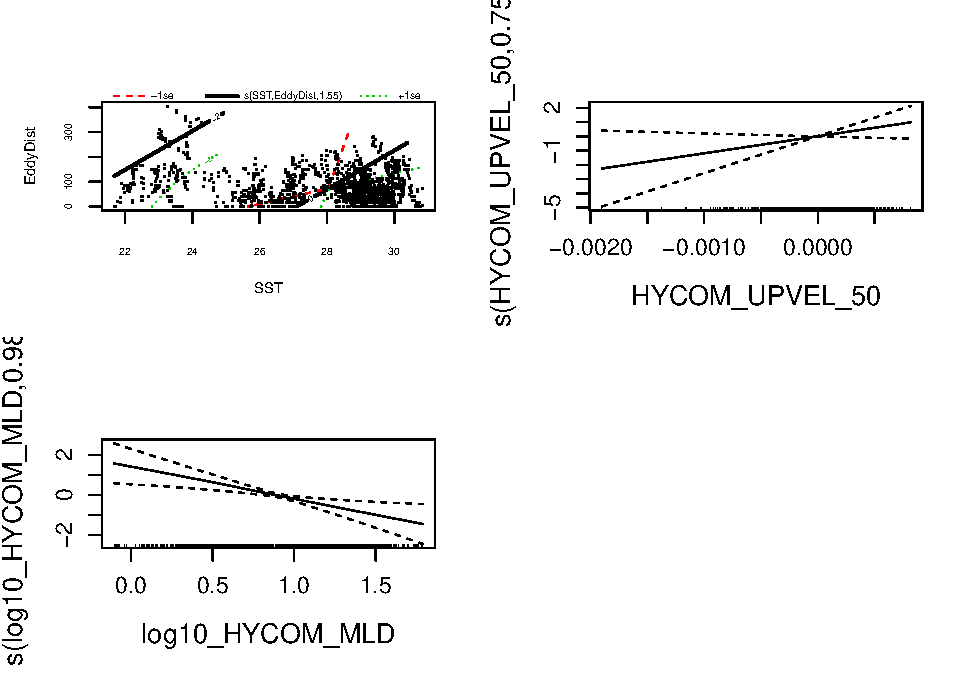
\includegraphics{Zc_model_runs_files/figure-latex/Vis best model summary-1.pdf}

\begin{Shaded}
\begin{Highlighting}[]
\KeywordTok{save}\NormalTok{(VisOnly_gamm_pruned_TF_best,}\DataTypeTok{file =} \KeywordTok{paste}\NormalTok{(outDir,SP,}\StringTok{'_best_VisOnly_binomial_model.Rdata'}\NormalTok{,}\DataTypeTok{sep=}\StringTok{''}\NormalTok{))}
\end{Highlighting}
\end{Shaded}

\begin{Shaded}
\begin{Highlighting}[]
\KeywordTok{plot}\NormalTok{(}\KeywordTok{residuals.gam}\NormalTok{(VisOnly_gamm_pruned_TF_best$gam))}
\end{Highlighting}
\end{Shaded}

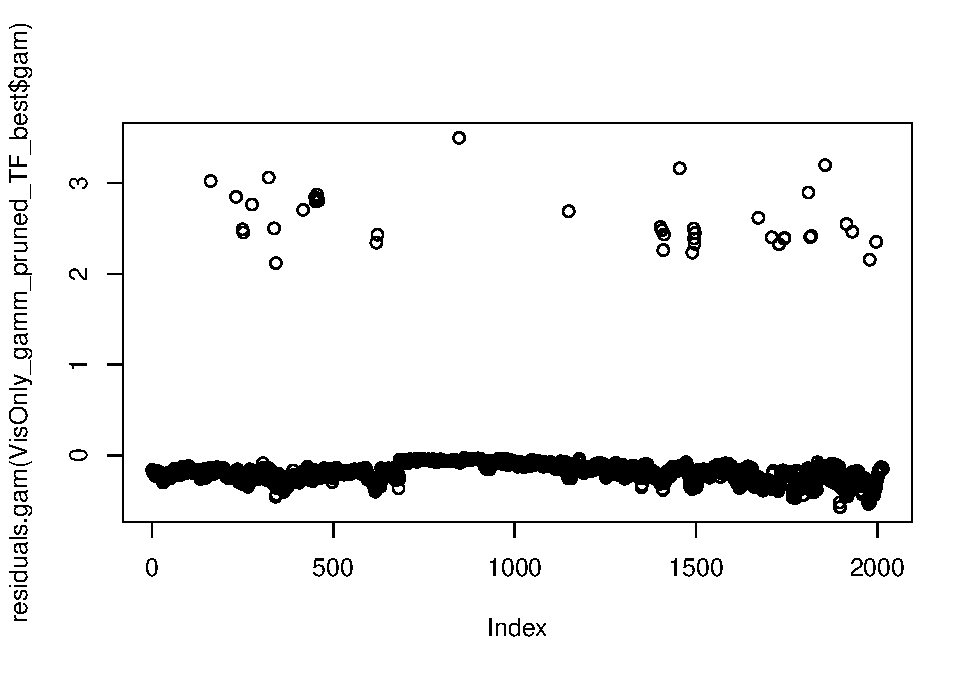
\includegraphics{Zc_model_runs_files/figure-latex/Vis best model residuals-1.pdf}

\begin{Shaded}
\begin{Highlighting}[]
\CommentTok{# gam.check(VisOnly_gamm_pruned_TF_best$gam)}
\end{Highlighting}
\end{Shaded}

\subsection{Best Joint Visual \& Acoustic
Model}\label{best-joint-visual-acoustic-model}

\begin{Shaded}
\begin{Highlighting}[]
\KeywordTok{summary}\NormalTok{(best_model$gam)}
\end{Highlighting}
\end{Shaded}

\begin{verbatim}
## 
## Family: quasibinomial 
## Link function: logit 
## 
## Formula:
## y_TF ~ s(SST, bs = "ts", k = kVal) + s(HYCOM_UPVEL_50, bs = "ts", 
##     k = kVal) + s(SSH, EddyDist, bs = "ts", k = kVal) + s(HYCOM_SALIN_0, 
##     bs = "ts", k = kVal) + s(log10_HYCOM_MLD, bs = "ts", k = kVal)
## 
## Parametric coefficients:
##             Estimate Std. Error t value Pr(>|t|)    
## (Intercept) -0.78286    0.06677  -11.72   <2e-16 ***
## ---
## Signif. codes:  0 '***' 0.001 '**' 0.01 '*' 0.05 '.' 0.1 ' ' 1
## 
## Approximate significance of smooth terms:
##                          edf Ref.df      F  p-value    
## s(SST)             3.381e+00      4 12.439 1.19e-11 ***
## s(HYCOM_UPVEL_50)  5.626e-06      4  0.000    0.972    
## s(SSH,EddyDist)    1.766e+00      4  4.390 4.64e-05 ***
## s(HYCOM_SALIN_0)   1.529e+00      4 60.438  < 2e-16 ***
## s(log10_HYCOM_MLD) 2.174e-01      4  0.091    0.193    
## ---
## Signif. codes:  0 '***' 0.001 '**' 0.01 '*' 0.05 '.' 0.1 ' ' 1
## 
## R-sq.(adj) =  0.206   
##   Scale est. = 0.95736   n = 3557
\end{verbatim}

Re-run the best joint model with only the significant terms

\begin{Shaded}
\begin{Highlighting}[]
\NormalTok{gamm_pruned_TF_best <-}\StringTok{ }\KeywordTok{gamm}\NormalTok{(y_TF~}\StringTok{ }\KeywordTok{s}\NormalTok{(SST, }\DataTypeTok{bs=}\StringTok{'ts'}\NormalTok{, }\DataTypeTok{k=}\NormalTok{kVal) }
                        \NormalTok{+}\StringTok{ }\KeywordTok{s}\NormalTok{(HYCOM_SALIN_0, }\DataTypeTok{bs=}\StringTok{'ts'}\NormalTok{, }\DataTypeTok{k=}\NormalTok{kVal)}
                        \NormalTok{+}\StringTok{ }\KeywordTok{s}\NormalTok{(SSH,EddyDist,}\DataTypeTok{bs=}\StringTok{'ts'}\NormalTok{, }\DataTypeTok{k=}\NormalTok{kVal),}
                        \DataTypeTok{data =} \NormalTok{transformedCovars.train, }
                        \DataTypeTok{weights =} \NormalTok{mergedTrain.set$Weight/}\KeywordTok{mean}\NormalTok{(mergedTrain.set$Weight),}
                        \DataTypeTok{na.action =} \NormalTok{na.omit,}\DataTypeTok{family =} \KeywordTok{quasibinomial}\NormalTok{(),}
                        \DataTypeTok{correlation =} \KeywordTok{corAR1}\NormalTok{(}\DataTypeTok{form=}\NormalTok{~}\DecValTok{1}\NormalTok{|fac2),}\DataTypeTok{niterPQL =} \DecValTok{30}\NormalTok{)}
\end{Highlighting}
\end{Shaded}

\begin{Shaded}
\begin{Highlighting}[]
\KeywordTok{summary}\NormalTok{(gamm_pruned_TF_best$gam)}
\end{Highlighting}
\end{Shaded}

\begin{verbatim}
## 
## Family: quasibinomial 
## Link function: logit 
## 
## Formula:
## y_TF ~ s(SST, bs = "ts", k = kVal) + s(HYCOM_SALIN_0, bs = "ts", 
##     k = kVal) + s(SSH, EddyDist, bs = "ts", k = kVal)
## 
## Parametric coefficients:
##             Estimate Std. Error t value Pr(>|t|)    
## (Intercept) -0.78098    0.06672  -11.71   <2e-16 ***
## ---
## Signif. codes:  0 '***' 0.001 '**' 0.01 '*' 0.05 '.' 0.1 ' ' 1
## 
## Approximate significance of smooth terms:
##                    edf Ref.df      F  p-value    
## s(SST)           3.389      4 12.361 2.05e-11 ***
## s(HYCOM_SALIN_0) 1.531      4 61.443  < 2e-16 ***
## s(SSH,EddyDist)  1.759      4  4.242 6.34e-05 ***
## ---
## Signif. codes:  0 '***' 0.001 '**' 0.01 '*' 0.05 '.' 0.1 ' ' 1
## 
## R-sq.(adj) =  0.206   
##   Scale est. = 0.95651   n = 3557
\end{verbatim}

\begin{Shaded}
\begin{Highlighting}[]
\KeywordTok{plot}\NormalTok{(gamm_pruned_TF_best$gam,}\DataTypeTok{pages=}\DecValTok{1}\NormalTok{,}\DataTypeTok{cex.lab =} \FloatTok{1.3}\NormalTok{,}\DataTypeTok{cex.axis =} \FloatTok{1.1}\NormalTok{,}\DataTypeTok{scale=}\DecValTok{0}\NormalTok{)}
\end{Highlighting}
\end{Shaded}

\includegraphics{Zc_model_runs_files/figure-latex/best model summary-1.pdf}

\begin{Shaded}
\begin{Highlighting}[]
\KeywordTok{save}\NormalTok{(gamm_pruned_TF_best,}\DataTypeTok{file =} \KeywordTok{paste}\NormalTok{(outDir,SP,}\StringTok{'_best_joint_binomial_model.Rdata'}\NormalTok{,}\DataTypeTok{sep=}\StringTok{''}\NormalTok{))}
\end{Highlighting}
\end{Shaded}

\begin{Shaded}
\begin{Highlighting}[]
\KeywordTok{plot}\NormalTok{(}\KeywordTok{residuals.gam}\NormalTok{(gamm_pruned_TF_best$gam))}
\end{Highlighting}
\end{Shaded}

\includegraphics{Zc_model_runs_files/figure-latex/best model residuals-1.pdf}

\begin{Shaded}
\begin{Highlighting}[]
\CommentTok{# gam.check(gamm_pruned_TF_best$gam)}
\end{Highlighting}
\end{Shaded}

\section{IV. Predict on Test Data}\label{iv.-predict-on-test-data}

\subsection{Temporal prediction}\label{temporal-prediction}

\subsubsection{Acoustic Only Model}\label{acoustic-only-model}

Predict on acoustic test data, and compare with actual observations for
2013. We are comparing the predicted probability of encountering animals
with the actual weekly rate of occurrence of animals at a site.

CAVEAT: Encounter probability from the data is estimated as fraction of
days per week during which Risso's were detected. This results in a
pretty coarse estimate. Alternatively we could compare to daily
densities or something, but then the y-axis scales are completely
different and it may be an apples to oranges comparison. An earlier
version used densities, and seemed to suggest that lagging variables
might be appropriate\ldots{}

\begin{Shaded}
\begin{Highlighting}[]
\CommentTok{# Predict on acoustic test data, using acoustic only model for comparison...}
\NormalTok{compAcSet_MC <-}\StringTok{ }\KeywordTok{which}\NormalTok{((Test_AcOnly.set$fac2)==}\DecValTok{5}\NormalTok{)}
\NormalTok{compAcSet_GC <-}\StringTok{ }\KeywordTok{which}\NormalTok{((Test_AcOnly.set$fac2)==}\DecValTok{10}\NormalTok{)}
\NormalTok{compAcSet_DT <-}\StringTok{ }\KeywordTok{which}\NormalTok{((Test_AcOnly.set$fac2)==}\DecValTok{15} \NormalTok{|}
\StringTok{                        }\NormalTok{(Test_AcOnly.set$fac2)==}\DecValTok{16}\NormalTok{)}

\CommentTok{# Predict in time}
\NormalTok{dateTicks =}\StringTok{ }\KeywordTok{as.POSIXct}\NormalTok{(}\KeywordTok{c}\NormalTok{(}\StringTok{'2013-01-01 GMT'}\NormalTok{,}\StringTok{'2013-04-01 GMT'}\NormalTok{,}
                         \StringTok{'2013-07-01 GMT'}\NormalTok{,}\StringTok{'2013-10-01 GMT'}\NormalTok{,}
                         \StringTok{'2014-01-01 GMT'}\NormalTok{))}
\NormalTok{dateLabels =}\StringTok{ }\KeywordTok{c}\NormalTok{(}\StringTok{'Jan. 2013'}\NormalTok{,}\StringTok{'Apr. 2013'}\NormalTok{,}\StringTok{'Jul. 2013'}\NormalTok{,}\StringTok{'Oct 2013'}\NormalTok{,}\StringTok{'Jan. 2014'}\NormalTok{)}
\NormalTok{predAcOnly_MC <-}\StringTok{ }\KeywordTok{predict.gam}\NormalTok{(AcOnly_gamm_pruned_TF_best$gam,}
                             \NormalTok{transformedCovars_AcOnly.test[compAcSet_MC,],}
                             \DataTypeTok{type =} \StringTok{'response'}\NormalTok{,}\DataTypeTok{na.action =} \NormalTok{na.pass)}
\NormalTok{predAcOnly_GC <-}\StringTok{ }\KeywordTok{predict.gam}\NormalTok{(AcOnly_gamm_pruned_TF_best$gam,}
                             \NormalTok{transformedCovars_AcOnly.test[compAcSet_GC,],}
                             \DataTypeTok{type =} \StringTok{'response'}\NormalTok{,}\DataTypeTok{na.action =} \NormalTok{na.pass)}
\NormalTok{predAcOnly_DT <-}\StringTok{ }\KeywordTok{predict.gam}\NormalTok{(AcOnly_gamm_pruned_TF_best$gam,}
                             \NormalTok{transformedCovars_AcOnly.test[compAcSet_DT,],}
                            \DataTypeTok{type =} \StringTok{'response'}\NormalTok{,}\DataTypeTok{na.action =} \NormalTok{na.pass)}

\NormalTok{occurIdx =}\StringTok{ }\KeywordTok{which}\NormalTok{(}\KeywordTok{as.POSIXct}\NormalTok{(pOccur[,}\DecValTok{1}\NormalTok{])>=}\StringTok{'2013-01-01'} \NormalTok{&}\StringTok{ }\KeywordTok{as.POSIXct}\NormalTok{(pOccur[,}\DecValTok{1}\NormalTok{])<}\StringTok{'2014-01-01'}\NormalTok{)}


\NormalTok{AcOnly_predictionSet <-}\StringTok{ }\KeywordTok{data.frame}\NormalTok{(}\KeywordTok{unique}\NormalTok{(Test_AcOnly.set$date))}
\KeywordTok{colnames}\NormalTok{(AcOnly_predictionSet) <-}\StringTok{"date"}
\NormalTok{AcOnly_predictionSet$MC <-}\StringTok{ }\OtherTok{NA}
\NormalTok{MC_times <-}\StringTok{ }\NormalTok{Test_AcOnly.set$date[compAcSet_MC]}
\NormalTok{m1 <-}\StringTok{ }\KeywordTok{match}\NormalTok{(MC_times,AcOnly_predictionSet$date)}
\NormalTok{AcOnly_predictionSet$MC[m1] <-predAcOnly_MC}

\NormalTok{AcOnly_predictionSet$GC <-}\StringTok{ }\OtherTok{NA}
\NormalTok{GC_times <-}\StringTok{ }\NormalTok{Test_AcOnly.set$date[compAcSet_GC]}
\NormalTok{m2 <-}\StringTok{ }\KeywordTok{match}\NormalTok{(GC_times,AcOnly_predictionSet$date)}
\NormalTok{AcOnly_predictionSet$GC[m2] <-predAcOnly_GC}

\NormalTok{AcOnly_predictionSet$DT <-}\StringTok{ }\OtherTok{NA}
\NormalTok{DT_times <-}\StringTok{ }\NormalTok{Test_AcOnly.set$date[compAcSet_DT]}
\NormalTok{m3 <-}\StringTok{ }\KeywordTok{match}\NormalTok{(DT_times,AcOnly_predictionSet$date)}
\NormalTok{AcOnly_predictionSet$DT[m3] <-predAcOnly_DT}

\NormalTok{AcOnly_predictionSet$Legend <-}\StringTok{ "Predictions"}

\NormalTok{pOccur$Legend <-}\StringTok{ "Observations"}
\end{Highlighting}
\end{Shaded}

\begin{Shaded}
\begin{Highlighting}[]
\CommentTok{# par(mfrow = c(5,1),oma=c(3,0,5,0)),colour="#000099",colour="#CC0000"}
\NormalTok{p1_Ac <-}\StringTok{ }\KeywordTok{ggplot}\NormalTok{() +}
\StringTok{  }\KeywordTok{geom_line}\NormalTok{(}\DataTypeTok{data =} \NormalTok{pOccur[occurIdx,],}
             \KeywordTok{aes}\NormalTok{(}\DataTypeTok{x =} \KeywordTok{as.POSIXct}\NormalTok{(dateStr), }\DataTypeTok{y =} \NormalTok{MC, }\DataTypeTok{color =} \NormalTok{Legend))+}
\StringTok{  }\KeywordTok{geom_line}\NormalTok{(}\DataTypeTok{data =} \NormalTok{AcOnly_predictionSet,}
            \KeywordTok{aes}\NormalTok{(}\DataTypeTok{x=}\NormalTok{date, }\DataTypeTok{y=}\NormalTok{MC, }\DataTypeTok{color =} \NormalTok{Legend)) +}
\StringTok{  }\KeywordTok{labs}\NormalTok{(}\DataTypeTok{y =} \StringTok{""}\NormalTok{, }\DataTypeTok{x =} \StringTok{""}\NormalTok{)+}
\StringTok{  }\KeywordTok{scale_color_manual}\NormalTok{(}\StringTok{""}\NormalTok{,}\DataTypeTok{values=} \KeywordTok{c}\NormalTok{(}\StringTok{"gray48"}\NormalTok{,}\StringTok{"#009999"}\NormalTok{))+}
\StringTok{  }\KeywordTok{theme}\NormalTok{(}\DataTypeTok{legend.position =} \KeywordTok{c}\NormalTok{(}\FloatTok{0.9}\NormalTok{, }\FloatTok{0.7}\NormalTok{))}

\NormalTok{p2_Ac <-}\StringTok{ }\KeywordTok{ggplot}\NormalTok{() +}
\StringTok{  }\KeywordTok{geom_line}\NormalTok{(}\DataTypeTok{data =} \NormalTok{pOccur[occurIdx,],}
             \KeywordTok{aes}\NormalTok{(}\DataTypeTok{x =}\KeywordTok{as.POSIXct}\NormalTok{(dateStr), }\DataTypeTok{y =} \NormalTok{GC, }\DataTypeTok{color =} \NormalTok{Legend))+}
\StringTok{  }\KeywordTok{geom_line}\NormalTok{(}\DataTypeTok{data =} \NormalTok{AcOnly_predictionSet,}
            \KeywordTok{aes}\NormalTok{(}\DataTypeTok{x=}\NormalTok{date, }\DataTypeTok{y=}\NormalTok{GC, }\DataTypeTok{color =} \NormalTok{Legend))+}
\StringTok{  }\KeywordTok{scale_color_manual}\NormalTok{(}\StringTok{""}\NormalTok{,}\DataTypeTok{values=} \KeywordTok{c}\NormalTok{(}\StringTok{"gray48"}\NormalTok{,}\StringTok{"#009999"}\NormalTok{))+}
\StringTok{  }\KeywordTok{labs}\NormalTok{(}\DataTypeTok{y =} \StringTok{""}\NormalTok{, }\DataTypeTok{x =} \StringTok{""}\NormalTok{)+}
\StringTok{  }\KeywordTok{theme}\NormalTok{(}\DataTypeTok{legend.position=}\StringTok{"none"}\NormalTok{)}

\NormalTok{p3_Ac <-}\StringTok{ }\KeywordTok{ggplot}\NormalTok{() +}
\StringTok{  }\KeywordTok{geom_line}\NormalTok{(}\DataTypeTok{data =} \NormalTok{pOccur[occurIdx,],}
             \KeywordTok{aes}\NormalTok{(}\DataTypeTok{x =}\KeywordTok{as.POSIXct}\NormalTok{(dateStr), }\DataTypeTok{y =} \NormalTok{DT, }\DataTypeTok{color =} \NormalTok{Legend))+}
\StringTok{  }\KeywordTok{geom_line}\NormalTok{(}\DataTypeTok{data =} \NormalTok{AcOnly_predictionSet,}
            \KeywordTok{aes}\NormalTok{(}\DataTypeTok{x=}\NormalTok{date, }\DataTypeTok{y=}\NormalTok{DT, }\DataTypeTok{color =} \NormalTok{Legend)) +}
\StringTok{  }\KeywordTok{scale_color_manual}\NormalTok{(}\StringTok{""}\NormalTok{,}\DataTypeTok{values=} \KeywordTok{c}\NormalTok{(}\StringTok{"gray48"}\NormalTok{,}\StringTok{"#009999"}\NormalTok{))+}
\StringTok{  }\KeywordTok{labs}\NormalTok{(}\DataTypeTok{y =} \StringTok{"Encounter probability"}\NormalTok{, }\DataTypeTok{x =} \StringTok{""}\NormalTok{)+}
\StringTok{  }\KeywordTok{theme}\NormalTok{(}\DataTypeTok{legend.position=}\StringTok{"none"}\NormalTok{)}


\KeywordTok{multiplot}\NormalTok{(p1_Ac, p2_Ac, p3_Ac, }\DataTypeTok{cols=}\DecValTok{1}\NormalTok{)}
\end{Highlighting}
\end{Shaded}

\includegraphics{Zc_model_runs_files/figure-latex/unnamed-chunk-1-1.pdf}

\subsubsection{Visual Only Model}\label{visual-only-model}

\begin{Shaded}
\begin{Highlighting}[]
\CommentTok{# Confusing, but acoustic only predictors are passed in to since}
\CommentTok{# we're predicting on the acoustic timeseries.}
\NormalTok{predVisOnly_MC <-}\StringTok{ }\KeywordTok{predict.gam}\NormalTok{(VisOnly_gamm_pruned_TF_best$gam,}
                              \NormalTok{transformedCovars_AcOnly.test[compAcSet_MC,],}
                              \DataTypeTok{type =} \StringTok{'response'}\NormalTok{,}\DataTypeTok{na.action =} \NormalTok{na.pass)}
\NormalTok{predVisOnly_GC <-}\StringTok{ }\KeywordTok{predict.gam}\NormalTok{(VisOnly_gamm_pruned_TF_best$gam,}
                              \NormalTok{transformedCovars_AcOnly.test[compAcSet_GC,],}
                              \DataTypeTok{type =} \StringTok{'response'}\NormalTok{,}\DataTypeTok{na.action =} \NormalTok{na.pass)}
\NormalTok{predVisOnly_DT <-}\StringTok{ }\KeywordTok{predict.gam}\NormalTok{(VisOnly_gamm_pruned_TF_best$gam,}
                              \NormalTok{transformedCovars_AcOnly.test[compAcSet_DT,],}
                              \DataTypeTok{type =} \StringTok{'response'}\NormalTok{,}\DataTypeTok{na.action =} \NormalTok{na.pass)}

\NormalTok{VisOnly_predictionSet <-}\StringTok{ }\KeywordTok{data.frame}\NormalTok{(}\KeywordTok{unique}\NormalTok{(Test_AcOnly.set$date))}
\KeywordTok{colnames}\NormalTok{(VisOnly_predictionSet) <-}\StringTok{"date"}
\NormalTok{VisOnly_predictionSet$MC <-}\StringTok{ }\OtherTok{NA}
\NormalTok{m1 <-}\StringTok{ }\KeywordTok{match}\NormalTok{(MC_times,VisOnly_predictionSet$date)}
\NormalTok{VisOnly_predictionSet$MC[m1] <-predVisOnly_MC}

\NormalTok{VisOnly_predictionSet$GC <-}\StringTok{ }\OtherTok{NA}
\NormalTok{m2 <-}\StringTok{ }\KeywordTok{match}\NormalTok{(GC_times,VisOnly_predictionSet$date)}
\NormalTok{VisOnly_predictionSet$GC[m2] <-predVisOnly_GC}

\NormalTok{VisOnly_predictionSet$DT <-}\StringTok{ }\OtherTok{NA}
\NormalTok{m3 <-}\StringTok{ }\KeywordTok{match}\NormalTok{(DT_times,VisOnly_predictionSet$date)}
\NormalTok{VisOnly_predictionSet$DT[m3] <-predVisOnly_DT}

\NormalTok{VisOnly_predictionSet$Legend <-}\StringTok{ "Predictions"}
\end{Highlighting}
\end{Shaded}

\begin{Shaded}
\begin{Highlighting}[]
\CommentTok{# par(mfrow = c(5,1),oma=c(3,0,5,0)),colour="#000099",colour="#CC0000"}
\NormalTok{p1_Vis <-}\StringTok{ }\KeywordTok{ggplot}\NormalTok{() +}
\StringTok{  }\KeywordTok{geom_line}\NormalTok{(}\DataTypeTok{data =} \NormalTok{pOccur[occurIdx,],}
             \KeywordTok{aes}\NormalTok{(}\DataTypeTok{x =} \KeywordTok{as.POSIXct}\NormalTok{(dateStr), }\DataTypeTok{y =} \NormalTok{MC, }\DataTypeTok{color =} \NormalTok{Legend))+}
\StringTok{  }\KeywordTok{geom_line}\NormalTok{(}\DataTypeTok{data =} \NormalTok{VisOnly_predictionSet,}
            \KeywordTok{aes}\NormalTok{(}\DataTypeTok{x=}\NormalTok{date, }\DataTypeTok{y=}\NormalTok{MC, }\DataTypeTok{color =} \NormalTok{Legend)) +}
\StringTok{  }\KeywordTok{labs}\NormalTok{(}\DataTypeTok{y =} \StringTok{""}\NormalTok{, }\DataTypeTok{x =} \StringTok{""}\NormalTok{)+}
\StringTok{  }\KeywordTok{scale_color_manual}\NormalTok{(}\DataTypeTok{values=} \KeywordTok{c}\NormalTok{(}\StringTok{"gray48"}\NormalTok{,}\StringTok{"#009999"}\NormalTok{))+}
\StringTok{  }\KeywordTok{theme}\NormalTok{(}\DataTypeTok{legend.position =} \KeywordTok{c}\NormalTok{(}\FloatTok{0.9}\NormalTok{, }\FloatTok{0.7}\NormalTok{))}

\NormalTok{p2_Vis <-}\StringTok{ }\KeywordTok{ggplot}\NormalTok{() +}
\StringTok{  }\KeywordTok{geom_line}\NormalTok{(}\DataTypeTok{data =} \NormalTok{pOccur[occurIdx,],}
             \KeywordTok{aes}\NormalTok{(}\DataTypeTok{x =}\KeywordTok{as.POSIXct}\NormalTok{(dateStr), }\DataTypeTok{y =} \NormalTok{GC, }\DataTypeTok{color =} \NormalTok{Legend))+}
\StringTok{  }\KeywordTok{geom_line}\NormalTok{(}\DataTypeTok{data =} \NormalTok{VisOnly_predictionSet,}
            \KeywordTok{aes}\NormalTok{(}\DataTypeTok{x=}\NormalTok{date, }\DataTypeTok{y=}\NormalTok{GC, }\DataTypeTok{color =} \NormalTok{Legend)) +}
\StringTok{  }\KeywordTok{scale_color_manual}\NormalTok{(}\DataTypeTok{values=} \KeywordTok{c}\NormalTok{(}\StringTok{"gray48"}\NormalTok{,}\StringTok{"#009999"}\NormalTok{))+}
\StringTok{  }\KeywordTok{labs}\NormalTok{(}\DataTypeTok{y =} \StringTok{""}\NormalTok{, }\DataTypeTok{x =} \StringTok{""}\NormalTok{)+}
\StringTok{  }\KeywordTok{theme}\NormalTok{(}\DataTypeTok{legend.position=}\StringTok{"none"}\NormalTok{)}

\NormalTok{p3_Vis <-}\StringTok{ }\KeywordTok{ggplot}\NormalTok{() +}
\StringTok{  }\KeywordTok{geom_line}\NormalTok{(}\DataTypeTok{data =} \NormalTok{pOccur[occurIdx,],}
             \KeywordTok{aes}\NormalTok{(}\DataTypeTok{x =}\KeywordTok{as.POSIXct}\NormalTok{(dateStr), }\DataTypeTok{y =} \NormalTok{DT, }\DataTypeTok{color =} \NormalTok{Legend))+}
\StringTok{    }\KeywordTok{geom_line}\NormalTok{(}\DataTypeTok{data =} \NormalTok{VisOnly_predictionSet,}
            \KeywordTok{aes}\NormalTok{(}\DataTypeTok{x=}\NormalTok{date, }\DataTypeTok{y=}\NormalTok{DT, }\DataTypeTok{color =} \NormalTok{Legend)) +}
\StringTok{  }\KeywordTok{scale_color_manual}\NormalTok{(}\DataTypeTok{values=} \KeywordTok{c}\NormalTok{(}\StringTok{"gray48"}\NormalTok{,}\StringTok{"#009999"}\NormalTok{))+}
\StringTok{  }\KeywordTok{labs}\NormalTok{(}\DataTypeTok{y =} \StringTok{"Encounter probability"}\NormalTok{, }\DataTypeTok{x =} \StringTok{""}\NormalTok{)+}
\StringTok{  }\KeywordTok{theme}\NormalTok{(}\DataTypeTok{legend.position=}\StringTok{"none"}\NormalTok{)}


\KeywordTok{multiplot}\NormalTok{(p1_Vis, p2_Vis, p3_Vis, }\DataTypeTok{cols=}\DecValTok{1}\NormalTok{)}
\end{Highlighting}
\end{Shaded}

\includegraphics{Zc_model_runs_files/figure-latex/unnamed-chunk-2-1.pdf}

\subsubsection{Joint Model}\label{joint-model}

\begin{Shaded}
\begin{Highlighting}[]
\CommentTok{# Confusing, but acoustic only predictors are passed in to since we're predicting on the acoustic timeseries.}
\NormalTok{pred_MC <-}\StringTok{ }\KeywordTok{predict.gam}\NormalTok{(gamm_pruned_TF_best$gam,}
                              \NormalTok{transformedCovars_AcOnly.test[compAcSet_MC,],}
                              \DataTypeTok{type =} \StringTok{'response'}\NormalTok{,}\DataTypeTok{na.action =} \NormalTok{na.pass)}
\NormalTok{pred_GC <-}\StringTok{ }\KeywordTok{predict.gam}\NormalTok{(gamm_pruned_TF_best$gam,}
                              \NormalTok{transformedCovars_AcOnly.test[compAcSet_GC,],}
                              \DataTypeTok{type =} \StringTok{'response'}\NormalTok{,}\DataTypeTok{na.action =} \NormalTok{na.pass)}
\NormalTok{pred_DT <-}\StringTok{ }\KeywordTok{predict.gam}\NormalTok{(gamm_pruned_TF_best$gam,}
                              \NormalTok{transformedCovars_AcOnly.test[compAcSet_DT,],}
                              \DataTypeTok{type =} \StringTok{'response'}\NormalTok{,}\DataTypeTok{na.action =} \NormalTok{na.pass)}

\NormalTok{Both_predictionSet <-}\StringTok{ }\KeywordTok{data.frame}\NormalTok{(}\KeywordTok{unique}\NormalTok{(Test_AcOnly.set$date))}
\KeywordTok{colnames}\NormalTok{(Both_predictionSet) <-}\StringTok{"date"}
\NormalTok{Both_predictionSet$MC <-}\StringTok{ }\OtherTok{NA}
\NormalTok{m1 <-}\StringTok{ }\KeywordTok{match}\NormalTok{(MC_times,Both_predictionSet$date)}
\NormalTok{Both_predictionSet$MC[m1] <-pred_MC}

\NormalTok{Both_predictionSet$GC <-}\StringTok{ }\OtherTok{NA}
\NormalTok{m2 <-}\StringTok{ }\KeywordTok{match}\NormalTok{(GC_times,Both_predictionSet$date)}
\NormalTok{Both_predictionSet$GC[m2] <-pred_GC}

\NormalTok{Both_predictionSet$DT <-}\StringTok{ }\OtherTok{NA}
\NormalTok{m3 <-}\StringTok{ }\KeywordTok{match}\NormalTok{(DT_times,Both_predictionSet$date)}
\NormalTok{Both_predictionSet$DT[m3] <-pred_DT}

\NormalTok{Both_predictionSet$Legend <-}\StringTok{ "Predictions"}
\end{Highlighting}
\end{Shaded}

\begin{Shaded}
\begin{Highlighting}[]
\CommentTok{# par(mfrow = c(5,1),oma=c(3,0,5,0)),colour="#000099",colour="#CC0000"}
\NormalTok{p1 <-}\StringTok{ }\KeywordTok{ggplot}\NormalTok{() +}
\StringTok{  }\KeywordTok{geom_line}\NormalTok{(}\DataTypeTok{data =} \NormalTok{pOccur[occurIdx,],}
             \KeywordTok{aes}\NormalTok{(}\DataTypeTok{x =} \KeywordTok{as.POSIXct}\NormalTok{(dateStr), }\DataTypeTok{y =} \NormalTok{MC, }\DataTypeTok{color =} \NormalTok{Legend))+}
\StringTok{  }\KeywordTok{geom_line}\NormalTok{(}\DataTypeTok{data =} \NormalTok{Both_predictionSet,}
            \KeywordTok{aes}\NormalTok{(}\DataTypeTok{x=}\NormalTok{date, }\DataTypeTok{y=}\NormalTok{MC, }\DataTypeTok{color =} \NormalTok{Legend)) +}
\StringTok{  }\KeywordTok{labs}\NormalTok{(}\DataTypeTok{y =} \StringTok{""}\NormalTok{, }\DataTypeTok{x =} \StringTok{""}\NormalTok{)+}
\StringTok{  }\KeywordTok{scale_color_manual}\NormalTok{(}\DataTypeTok{values=} \KeywordTok{c}\NormalTok{(}\StringTok{"gray48"}\NormalTok{,}\StringTok{"#009999"}\NormalTok{))+}
\StringTok{  }\KeywordTok{theme}\NormalTok{(}\DataTypeTok{legend.position =} \KeywordTok{c}\NormalTok{(}\FloatTok{0.9}\NormalTok{, }\FloatTok{0.7}\NormalTok{))}

\NormalTok{p2 <-}\StringTok{ }\KeywordTok{ggplot}\NormalTok{() +}
\StringTok{  }\KeywordTok{geom_line}\NormalTok{(}\DataTypeTok{data =} \NormalTok{pOccur[occurIdx,],}
             \KeywordTok{aes}\NormalTok{(}\DataTypeTok{x =}\KeywordTok{as.POSIXct}\NormalTok{(dateStr), }\DataTypeTok{y =} \NormalTok{GC, }\DataTypeTok{color =} \NormalTok{Legend))+}
\StringTok{  }\KeywordTok{geom_line}\NormalTok{(}\DataTypeTok{data =} \NormalTok{Both_predictionSet,}
            \KeywordTok{aes}\NormalTok{(}\DataTypeTok{x=}\NormalTok{date, }\DataTypeTok{y=}\NormalTok{GC, }\DataTypeTok{color =} \NormalTok{Legend)) +}
\StringTok{  }\KeywordTok{scale_color_manual}\NormalTok{(}\DataTypeTok{values=} \KeywordTok{c}\NormalTok{(}\StringTok{"gray48"}\NormalTok{,}\StringTok{"#009999"}\NormalTok{))+}
\StringTok{  }\KeywordTok{labs}\NormalTok{(}\DataTypeTok{y =} \StringTok{""}\NormalTok{, }\DataTypeTok{x =} \StringTok{""}\NormalTok{)+}
\StringTok{  }\KeywordTok{theme}\NormalTok{(}\DataTypeTok{legend.position=}\StringTok{"none"}\NormalTok{)}

\NormalTok{p3 <-}\StringTok{ }\KeywordTok{ggplot}\NormalTok{() +}
\StringTok{  }\KeywordTok{geom_line}\NormalTok{(}\DataTypeTok{data =} \NormalTok{pOccur[occurIdx,],}
             \KeywordTok{aes}\NormalTok{(}\DataTypeTok{x =}\KeywordTok{as.POSIXct}\NormalTok{(dateStr), }\DataTypeTok{y =} \NormalTok{DT, }\DataTypeTok{color =} \NormalTok{Legend))+}
\StringTok{  }\KeywordTok{geom_line}\NormalTok{(}\DataTypeTok{data =} \NormalTok{Both_predictionSet,}
            \KeywordTok{aes}\NormalTok{(}\DataTypeTok{x=}\NormalTok{date, }\DataTypeTok{y=}\NormalTok{DT, }\DataTypeTok{color =} \NormalTok{Legend)) +}
\StringTok{  }\KeywordTok{scale_color_manual}\NormalTok{(}\DataTypeTok{values=} \KeywordTok{c}\NormalTok{(}\StringTok{"gray48"}\NormalTok{,}\StringTok{"#009999"}\NormalTok{))+}
\StringTok{  }\KeywordTok{labs}\NormalTok{(}\DataTypeTok{y =} \StringTok{"Encounter probability"}\NormalTok{, }\DataTypeTok{x =} \StringTok{""}\NormalTok{)+}
\StringTok{  }\KeywordTok{theme}\NormalTok{(}\DataTypeTok{legend.position=}\StringTok{"none"}\NormalTok{)}

\KeywordTok{multiplot}\NormalTok{(p1, p2, p3, }\DataTypeTok{cols=}\DecValTok{1}\NormalTok{)}
\end{Highlighting}
\end{Shaded}

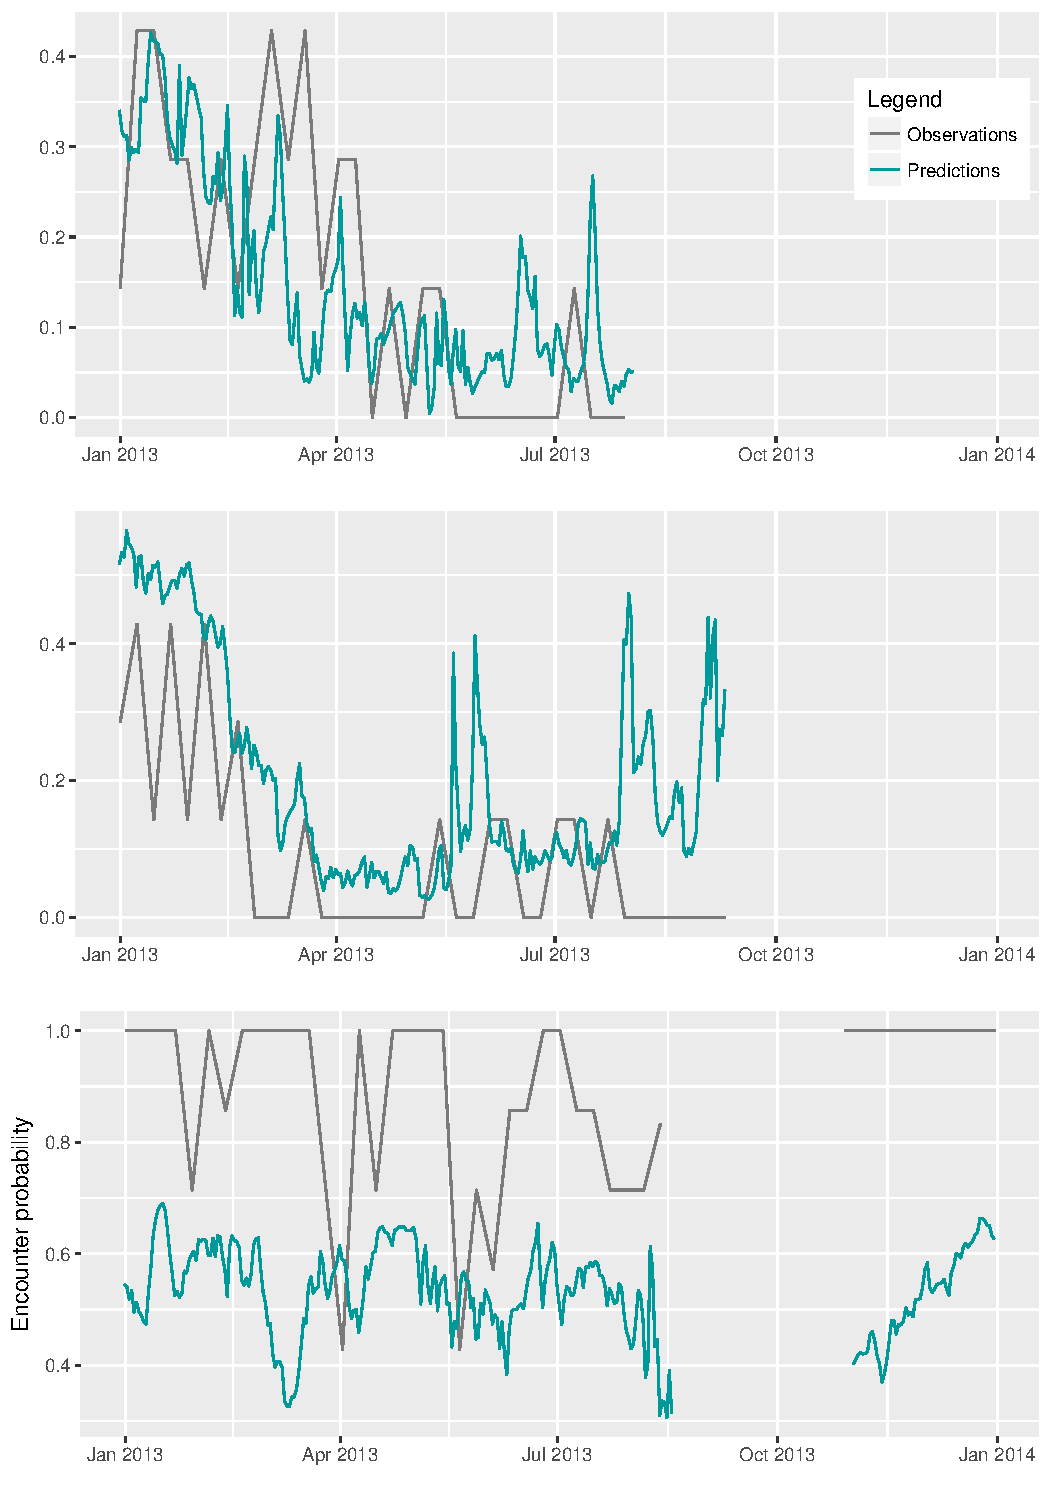
\includegraphics{Zc_model_runs_files/figure-latex/unnamed-chunk-3-1.pdf}

\subsection{Spatial Prediction}\label{spatial-prediction}

\subsubsection{Acoustic Only}\label{acoustic-only}

Evaluate the models for summer (July 2009) and winter(January 2009)
across the entire Gulf of Mexico (US EEZ beyond the 200m contour).

\begin{Shaded}
\begin{Highlighting}[]
\NormalTok{dt1 <-}\StringTok{ }\KeywordTok{as.data.frame}\NormalTok{(jan2009_rasters,}\DataTypeTok{xy=}\OtherTok{TRUE}\NormalTok{)}

\NormalTok{jan2009_AcOnly_prediction <-}\StringTok{ }\NormalTok{raster::}\KeywordTok{predict}\NormalTok{(jan2009_rasters,}
                                             \NormalTok{AcOnly_gamm_pruned_TF_best$gam,}
                                             \DataTypeTok{type =} \StringTok{'response'}\NormalTok{,}\DataTypeTok{na.action =} \NormalTok{na.pass)}
            
\NormalTok{july2009_AcOnly_prediction <-}\StringTok{ }\NormalTok{raster::}\KeywordTok{predict}\NormalTok{(july2009_rasters,}
                                              \NormalTok{AcOnly_gamm_pruned_TF_best$gam,}
                                              \DataTypeTok{type =} \StringTok{'response'}\NormalTok{,}\DataTypeTok{na.action =} \NormalTok{na.pass)    }
\end{Highlighting}
\end{Shaded}

\subsubsection{Visual Only}\label{visual-only}

\begin{Shaded}
\begin{Highlighting}[]
\NormalTok{dt1 <-}\StringTok{ }\KeywordTok{as.data.frame}\NormalTok{(jan2009_rasters,}\DataTypeTok{xy=}\OtherTok{TRUE}\NormalTok{)}

\NormalTok{jan2009_VisOnly_prediction <-}\StringTok{ }\NormalTok{raster::}\KeywordTok{predict}\NormalTok{(jan2009_rasters,VisOnly_gamm_pruned_TF_best$gam,}
            \DataTypeTok{type =} \StringTok{'response'}\NormalTok{,}\DataTypeTok{na.action =} \NormalTok{na.pass)}
            
\NormalTok{july2009_VisOnly_prediction <-}\StringTok{ }\NormalTok{raster::}\KeywordTok{predict}\NormalTok{(july2009_rasters,VisOnly_gamm_pruned_TF_best$gam,}
            \DataTypeTok{type =} \StringTok{'response'}\NormalTok{,}\DataTypeTok{na.action =} \NormalTok{na.pass)    }
\end{Highlighting}
\end{Shaded}

\subsubsection{Joint Visual and
Acoustic}\label{joint-visual-and-acoustic}

\begin{Shaded}
\begin{Highlighting}[]
\NormalTok{dt1 <-}\StringTok{ }\KeywordTok{as.data.frame}\NormalTok{(jan2009_rasters,}\DataTypeTok{xy=}\OtherTok{TRUE}\NormalTok{)}

\NormalTok{jan2009_prediction <-}\StringTok{ }\NormalTok{raster::}\KeywordTok{predict}\NormalTok{(jan2009_rasters,gamm_pruned_TF_best$gam,}
            \DataTypeTok{type =} \StringTok{'response'}\NormalTok{,}\DataTypeTok{na.action =} \NormalTok{na.pass)}
            
\NormalTok{july2009_prediction <-}\StringTok{ }\NormalTok{raster::}\KeywordTok{predict}\NormalTok{(july2009_rasters,gamm_pruned_TF_best$gam,}
            \DataTypeTok{type =} \StringTok{'response'}\NormalTok{,}\DataTypeTok{na.action =} \NormalTok{na.pass)    }
\end{Highlighting}
\end{Shaded}

Wrangle projections for mapping:

\begin{Shaded}
\begin{Highlighting}[]
\NormalTok{predict_template <-}\StringTok{ }\KeywordTok{readOGR}\NormalTok{(}\StringTok{'E:/NASData/AcoustoVisualDE/Prediction_template/prediction_polygon.shp'}\NormalTok{)}
\NormalTok{map_proj <-}\StringTok{ }\NormalTok{sp::}\KeywordTok{CRS}\NormalTok{(}\StringTok{'+proj=longlat +ellps=WGS84 +datum=WGS84 +no_defs'}\NormalTok{)}
\NormalTok{predict_template_proj <-}\StringTok{ }\KeywordTok{spTransform}\NormalTok{(predict_template, }\DataTypeTok{CRSobj =} \NormalTok{map_proj)}

\CommentTok{# Acoustic}
\NormalTok{jan2009_AcOnly_prediction_proj <-}\StringTok{ }\KeywordTok{projectRaster}\NormalTok{(jan2009_AcOnly_prediction, }\DataTypeTok{crs=}\NormalTok{map_proj)}
\NormalTok{july2009_AcOnly_prediction_proj <-}\StringTok{ }\KeywordTok{projectRaster}\NormalTok{(july2009_AcOnly_prediction, }\DataTypeTok{crs=}\NormalTok{map_proj)}
\NormalTok{jan2009_AcOnly_prediction_crop <-}\StringTok{ }\KeywordTok{mask}\NormalTok{(jan2009_AcOnly_prediction_proj,predict_template_proj)}
\NormalTok{july2009_AcOnly_prediction_crop <-}
\StringTok{  }\KeywordTok{mask}\NormalTok{(july2009_AcOnly_prediction_proj,predict_template_proj)}

\CommentTok{# Visual}
\NormalTok{jan2009_VisOnly_prediction_proj <-}\StringTok{ }
\StringTok{  }\KeywordTok{projectRaster}\NormalTok{(jan2009_VisOnly_prediction, }\DataTypeTok{crs=}\NormalTok{map_proj)}
\NormalTok{july2009_VisOnly_prediction_proj <-}\StringTok{ }
\StringTok{  }\KeywordTok{projectRaster}\NormalTok{(july2009_VisOnly_prediction, }\DataTypeTok{crs=}\NormalTok{map_proj)}
\CommentTok{#jan2009_VisOnly_prediction_SE_proj <- }
\CommentTok{#  projectRaster(jan2009_VisOnly_prediction_SE, crs=map_proj)}

\NormalTok{jan2009_VisOnly_prediction_crop <-}\StringTok{ }
\StringTok{  }\KeywordTok{mask}\NormalTok{(jan2009_VisOnly_prediction_proj,predict_template_proj)}
\NormalTok{july2009_VisOnly_prediction_crop <-}\StringTok{ }\KeywordTok{mask}\NormalTok{(july2009_VisOnly_prediction_proj,predict_template_proj)}
\CommentTok{#jan2009_VisOnly_prediction_SE_crop <- mask(jan2009_VisOnly_prediction_SE_proj,predict_template_proj)}

\CommentTok{#Both}
\NormalTok{jan2009_prediction_proj <-}\StringTok{ }\KeywordTok{projectRaster}\NormalTok{(jan2009_prediction, }\DataTypeTok{crs=}\NormalTok{map_proj)}
\NormalTok{july2009_prediction_proj <-}\StringTok{ }\KeywordTok{projectRaster}\NormalTok{(july2009_prediction, }\DataTypeTok{crs=}\NormalTok{map_proj)}
\NormalTok{jan2009_prediction_crop <-}\StringTok{ }\KeywordTok{mask}\NormalTok{(jan2009_prediction_proj,predict_template_proj)}
\NormalTok{july2009_prediction_crop <-}\StringTok{ }\KeywordTok{mask}\NormalTok{(july2009_prediction_proj,predict_template_proj)}
\end{Highlighting}
\end{Shaded}

\subsubsection{Model averaging}\label{model-averaging}

Alternatively, the visual and acoustic models could be averaged.

\begin{Shaded}
\begin{Highlighting}[]
\NormalTok{jan2009mean <-}\StringTok{ }\KeywordTok{mean}\NormalTok{(jan2009_AcOnly_prediction_crop,jan2009_VisOnly_prediction_crop)}
\NormalTok{july2009mean <-}\StringTok{ }\KeywordTok{mean}\NormalTok{(july2009_AcOnly_prediction_crop,july2009_VisOnly_prediction_crop)}
\end{Highlighting}
\end{Shaded}

Display summer (July 2009) map:

\begin{Shaded}
\begin{Highlighting}[]
\NormalTok{pal <-}\StringTok{ }\KeywordTok{colorNumeric}\NormalTok{(}\DataTypeTok{palette =} \KeywordTok{matlab.like2}\NormalTok{(}\DecValTok{5}\NormalTok{),}
                    \DataTypeTok{domain=}\KeywordTok{c}\NormalTok{(}\DecValTok{0}\NormalTok{,}\DecValTok{1}\NormalTok{), }
                    \DataTypeTok{na.color =} \StringTok{'transparent'}\NormalTok{)}

\NormalTok{map <-}\StringTok{ }\KeywordTok{leaflet}\NormalTok{() %>%}\StringTok{  }\KeywordTok{setView}\NormalTok{(}\DataTypeTok{lng =} \NormalTok{-}\FloatTok{88.8}\NormalTok{, }\DataTypeTok{lat =} \FloatTok{27.0}\NormalTok{, }\DataTypeTok{zoom =} \DecValTok{6}\NormalTok{)%>%}
\StringTok{  }\KeywordTok{addProviderTiles}\NormalTok{(providers$Esri.OceanBasemap) %>%}
\StringTok{  }\KeywordTok{addRasterImage}\NormalTok{(july2009_AcOnly_prediction_crop, }\DataTypeTok{colors =} \NormalTok{pal,}
                 \DataTypeTok{opacity =} \FloatTok{0.8}\NormalTok{, }\DataTypeTok{group =} \StringTok{'Acoustic July 2009'}\NormalTok{) %>%}
\StringTok{  }\KeywordTok{addRasterImage}\NormalTok{(july2009_VisOnly_prediction_crop, }\DataTypeTok{colors =} \NormalTok{pal,}
                 \DataTypeTok{opacity =} \FloatTok{0.8}\NormalTok{, }\DataTypeTok{group =} \StringTok{'Visual July 2009'}\NormalTok{) %>%}
\StringTok{  }\KeywordTok{addRasterImage}\NormalTok{(july2009_prediction_crop, }\DataTypeTok{colors =} \NormalTok{pal,}
                 \DataTypeTok{opacity =} \FloatTok{0.8}\NormalTok{, }\DataTypeTok{group =} \StringTok{'Joint July 2009'}\NormalTok{) %>%}
\StringTok{  }\KeywordTok{addRasterImage}\NormalTok{(july2009mean,}\DataTypeTok{colors =} \NormalTok{pal,}
                 \DataTypeTok{opacity =} \FloatTok{0.8}\NormalTok{, }\DataTypeTok{group =} \StringTok{'Vis. & Ac. Mean July 2009'}\NormalTok{) %>%}\StringTok{  }
\StringTok{  }\KeywordTok{addCircleMarkers}\NormalTok{(}\DataTypeTok{data =} \NormalTok{sightingsTest, }\DataTypeTok{lng =} \NormalTok{~}\StringTok{ }\NormalTok{long, }\DataTypeTok{lat =} \NormalTok{~}\StringTok{ }\NormalTok{lat,}\DataTypeTok{color =} \StringTok{"black"}\NormalTok{,}
                 \DataTypeTok{stroke =} \OtherTok{TRUE}\NormalTok{, }\DataTypeTok{fillOpacity =} \FloatTok{0.8}\NormalTok{,}\DataTypeTok{radius =} \DecValTok{6}\NormalTok{,}
                 \DataTypeTok{group =} \StringTok{'Test Sightings (Summer 2009)'}\NormalTok{) %>%}
\StringTok{  }\KeywordTok{addLegend}\NormalTok{(}\DataTypeTok{pal =} \NormalTok{pal, }\DataTypeTok{values =} \KeywordTok{c}\NormalTok{(}\DecValTok{0}\NormalTok{,}\DecValTok{1}\NormalTok{),}
    \DataTypeTok{title =} \StringTok{'P(encounter)'}\NormalTok{,}\DataTypeTok{position =} \StringTok{"bottomleft"}\NormalTok{) %>%}
\StringTok{  }\KeywordTok{addLayersControl}\NormalTok{(}
    \DataTypeTok{baseGroups =} \KeywordTok{c}\NormalTok{(}\StringTok{'Acoustic July 2009'}\NormalTok{,}\StringTok{'Visual July 2009'}\NormalTok{,}
                   \StringTok{'Joint July 2009'}\NormalTok{,}\StringTok{'Vis. & Ac. Mean July 2009'}\NormalTok{),}
    \DataTypeTok{overlayGroups =} \KeywordTok{c}\NormalTok{(}\StringTok{'Test Sightings (Summer 2009)'}\NormalTok{),}
    \DataTypeTok{options =} \KeywordTok{layersControlOptions}\NormalTok{(}\DataTypeTok{collapsed =} \OtherTok{FALSE}\NormalTok{)}
  \NormalTok{)}
\NormalTok{map}
\end{Highlighting}
\end{Shaded}

\hypertarget{htmlwidget-5f2928f6e74c02c741ba}{}

Display winter (January 2009) map:

\begin{Shaded}
\begin{Highlighting}[]
\NormalTok{pal <-}\StringTok{ }\KeywordTok{colorNumeric}\NormalTok{(}\DataTypeTok{palette =} \KeywordTok{matlab.like2}\NormalTok{(}\DecValTok{5}\NormalTok{),}
                    \DataTypeTok{domain=}\KeywordTok{c}\NormalTok{(}\DecValTok{0}\NormalTok{,}\DecValTok{1}\NormalTok{), }
                    \DataTypeTok{na.color =} \StringTok{'transparent'}\NormalTok{)}

\NormalTok{map <-}\StringTok{ }\KeywordTok{leaflet}\NormalTok{() %>%}\StringTok{  }\KeywordTok{setView}\NormalTok{(}\DataTypeTok{lng =} \NormalTok{-}\FloatTok{88.8}\NormalTok{, }\DataTypeTok{lat =} \FloatTok{27.0}\NormalTok{, }\DataTypeTok{zoom =} \DecValTok{6}\NormalTok{)%>%}
\StringTok{  }\KeywordTok{addProviderTiles}\NormalTok{(providers$Esri.OceanBasemap) %>%}
\StringTok{  }\KeywordTok{addRasterImage}\NormalTok{(jan2009_AcOnly_prediction_crop, }\DataTypeTok{colors =} \NormalTok{pal,}
                 \DataTypeTok{opacity =} \FloatTok{0.8}\NormalTok{, }\DataTypeTok{group =} \StringTok{'Acoustic Jan. 2009'}\NormalTok{) %>%}
\StringTok{  }\KeywordTok{addRasterImage}\NormalTok{(jan2009_VisOnly_prediction_crop, }\DataTypeTok{colors =} \NormalTok{pal,}
                 \DataTypeTok{opacity =} \FloatTok{0.8}\NormalTok{, }\DataTypeTok{group =} \StringTok{'Visual Jan. 2009'}\NormalTok{) %>%}
\StringTok{  }\KeywordTok{addRasterImage}\NormalTok{(jan2009_prediction_crop, }\DataTypeTok{colors =} \NormalTok{pal,}
                 \DataTypeTok{opacity =} \FloatTok{0.8}\NormalTok{, }\DataTypeTok{group =} \StringTok{'Joint Jan. 2009'}\NormalTok{) %>%}
\StringTok{  }\KeywordTok{addRasterImage}\NormalTok{(jan2009mean,}\DataTypeTok{colors =} \NormalTok{pal,}
                 \DataTypeTok{opacity =} \FloatTok{0.8}\NormalTok{, }\DataTypeTok{group =} \StringTok{'Vis. & Ac. Mean Jan. 2009'}\NormalTok{) %>%}
\StringTok{  }\KeywordTok{addLegend}\NormalTok{(}\DataTypeTok{pal =} \NormalTok{pal, }\DataTypeTok{values =} \KeywordTok{c}\NormalTok{(}\DecValTok{0}\NormalTok{,}\DecValTok{1}\NormalTok{),}
    \DataTypeTok{title =} \StringTok{'P(encounter)'}\NormalTok{,}\DataTypeTok{position =} \StringTok{"bottomleft"}\NormalTok{) %>%}
\StringTok{  }\KeywordTok{addLayersControl}\NormalTok{(}
    \DataTypeTok{baseGroups =} \KeywordTok{c}\NormalTok{(}\StringTok{'Acoustic Jan. 2009'}\NormalTok{,}\StringTok{'Visual Jan. 2009'}\NormalTok{,}
                   \StringTok{'Joint Jan. 2009'}\NormalTok{,}\StringTok{'Vis. & Ac. Mean Jan. 2009'}\NormalTok{),}
    \DataTypeTok{options =} \KeywordTok{layersControlOptions}\NormalTok{(}\DataTypeTok{collapsed =} \OtherTok{FALSE}\NormalTok{)}
  \NormalTok{)}
\NormalTok{map}
\end{Highlighting}
\end{Shaded}

\hypertarget{htmlwidget-d7b14bb34e6c4d069330}{}

\section{V. Monthly model
predictions}\label{v.-monthly-model-predictions}

Spatial model predictions using oceanographic variables averaged by
month between 2003 and 2015.

\begin{Shaded}
\begin{Highlighting}[]
\KeywordTok{load}\NormalTok{(}\StringTok{'E:/NASData/AcoustoVisualDE/AcoustoVisualDE/climatology_rasters.Rdata'}\NormalTok{) }
\NormalTok{monthNum <-}\KeywordTok{c}\NormalTok{(}\StringTok{'01'}\NormalTok{,}\StringTok{'02'}\NormalTok{,}\StringTok{'03'}\NormalTok{,}\StringTok{'04'}\NormalTok{,}\StringTok{'05'}\NormalTok{,}\StringTok{'06'}\NormalTok{,}\StringTok{'07'}\NormalTok{,}\StringTok{'08'}\NormalTok{,}\StringTok{'09'}\NormalTok{,}\StringTok{'10'}\NormalTok{,}\StringTok{'11'}\NormalTok{,}\StringTok{'12'}\NormalTok{)}
\NormalTok{monthStr<-}\KeywordTok{c}\NormalTok{(}\StringTok{'Jan'}\NormalTok{,}\StringTok{'Feb'}\NormalTok{,}\StringTok{'Mar'}\NormalTok{,}\StringTok{'Apr'}\NormalTok{,}\StringTok{'May'}\NormalTok{,}\StringTok{'Jun'}\NormalTok{,}\StringTok{'Jul'}\NormalTok{,}\StringTok{'Aug'}\NormalTok{,}\StringTok{'Sep'}\NormalTok{,}\StringTok{'Oct'}\NormalTok{,}\StringTok{'Nov'}\NormalTok{,}\StringTok{'Dec'}\NormalTok{)}

\NormalTok{climatePrediction <-}\StringTok{ }\KeywordTok{vector}\NormalTok{(}\StringTok{'list'}\NormalTok{,}\DataTypeTok{length =} \DecValTok{12}\NormalTok{)}
\NormalTok{mapClimatePrediction <-}\StringTok{ }\KeywordTok{vector}\NormalTok{(}\StringTok{'list'}\NormalTok{,}\DataTypeTok{length =} \DecValTok{12}\NormalTok{)}

\NormalTok{for (iM in }\DecValTok{1}\NormalTok{:}\KeywordTok{length}\NormalTok{(monthStr))\{}
  \NormalTok{climatePrediction[[iM]] <-}\StringTok{ }\NormalTok{raster::}\KeywordTok{predict}\NormalTok{(raster_set[[iM]],gamm_pruned_TF_best$gam,}
            \DataTypeTok{type =} \StringTok{'response'}\NormalTok{,}\DataTypeTok{na.action =} \NormalTok{na.pass)}
  \NormalTok{mapClimatePrediction[[iM]] <-}\StringTok{ }\KeywordTok{mask}\NormalTok{(}\KeywordTok{projectRaster}\NormalTok{(climatePrediction[[iM]], }\DataTypeTok{crs=}\NormalTok{map_proj),predict_template_proj)  }
  \CommentTok{# output raster to geotiff}
  \NormalTok{rasterImageFileName =}\StringTok{ }\KeywordTok{paste0}\NormalTok{(savePath,}\StringTok{'/climatology_predictions/'}\NormalTok{, SP,}\StringTok{'_'}\NormalTok{,monthStr[iM],}\StringTok{'_mean_encounter_probability.tif'}\NormalTok{)}
  \KeywordTok{writeRaster}\NormalTok{(mapClimatePrediction[[iM]],}\DataTypeTok{filename =} \NormalTok{rasterImageFileName, }\DataTypeTok{format=}\StringTok{"GTiff"}\NormalTok{,}\DataTypeTok{overwrite =} \OtherTok{TRUE}\NormalTok{)}
  
  \CommentTok{#ouput raster to kml}
  \NormalTok{kmlImageFileName =}\StringTok{ }\KeywordTok{paste0}\NormalTok{(savePath,}\StringTok{'/climatology_predictions/'}\NormalTok{, SP,}\StringTok{'_'}\NormalTok{,monthStr[iM],}\StringTok{'_mean_encounter_probability.kml'}\NormalTok{)}
  \KeywordTok{KML}\NormalTok{(mapClimatePrediction[[iM]],}\DataTypeTok{file =} \NormalTok{kmlImageFileName, }\DataTypeTok{col=}\KeywordTok{matlab.like2}\NormalTok{(}\DecValTok{32}\NormalTok{),}\DataTypeTok{overwrite =} \OtherTok{TRUE}\NormalTok{)}
  

\NormalTok{\}}
\end{Highlighting}
\end{Shaded}

\begin{Shaded}
\begin{Highlighting}[]
\NormalTok{pal <-}\StringTok{ }\KeywordTok{colorNumeric}\NormalTok{(}\DataTypeTok{palette =} \KeywordTok{matlab.like2}\NormalTok{(}\DecValTok{5}\NormalTok{),}
                    \DataTypeTok{domain=}\KeywordTok{c}\NormalTok{(}\DecValTok{0}\NormalTok{,.}\DecValTok{8}\NormalTok{), }
                    \DataTypeTok{na.color =} \StringTok{'transparent'}\NormalTok{)}

\NormalTok{map <-}\StringTok{ }\KeywordTok{leaflet}\NormalTok{() %>%}\StringTok{  }\KeywordTok{setView}\NormalTok{(}\DataTypeTok{lng =} \NormalTok{-}\FloatTok{88.8}\NormalTok{, }\DataTypeTok{lat =} \FloatTok{27.0}\NormalTok{, }\DataTypeTok{zoom =} \DecValTok{6}\NormalTok{)%>%}
\StringTok{  }\KeywordTok{addProviderTiles}\NormalTok{(providers$Esri.OceanBasemap) %>%}
\StringTok{  }\KeywordTok{addRasterImage}\NormalTok{(mapClimatePrediction[[}\DecValTok{1}\NormalTok{]] , }\DataTypeTok{colors =} \NormalTok{pal,}
                 \DataTypeTok{opacity =} \FloatTok{0.8}\NormalTok{, }\DataTypeTok{group =} \StringTok{'Jan.'}\NormalTok{) %>%}
\StringTok{  }\KeywordTok{addRasterImage}\NormalTok{(mapClimatePrediction[[}\DecValTok{4}\NormalTok{]] , }\DataTypeTok{colors =} \NormalTok{pal,}
                 \DataTypeTok{opacity =} \FloatTok{0.8}\NormalTok{, }\DataTypeTok{group =} \StringTok{'April'}\NormalTok{) %>%}
\StringTok{  }\KeywordTok{addRasterImage}\NormalTok{(mapClimatePrediction[[}\DecValTok{7}\NormalTok{]] , }\DataTypeTok{colors =} \NormalTok{pal,}
                 \DataTypeTok{opacity =} \FloatTok{0.8}\NormalTok{, }\DataTypeTok{group =} \StringTok{'July'}\NormalTok{) %>%}
\StringTok{  }\KeywordTok{addRasterImage}\NormalTok{(mapClimatePrediction[[}\DecValTok{10}\NormalTok{]] ,}\DataTypeTok{colors =} \NormalTok{pal,}
                 \DataTypeTok{opacity =} \FloatTok{0.8}\NormalTok{, }\DataTypeTok{group =} \StringTok{'Oct.'}\NormalTok{) %>%}
\StringTok{  }\KeywordTok{addLegend}\NormalTok{(}\DataTypeTok{pal =} \NormalTok{pal, }\DataTypeTok{values =} \KeywordTok{c}\NormalTok{(}\DecValTok{0}\NormalTok{,.}\DecValTok{8}\NormalTok{),}
    \DataTypeTok{title =} \StringTok{'P(encounter)'}\NormalTok{,}\DataTypeTok{position =} \StringTok{"bottomleft"}\NormalTok{) %>%}
\StringTok{  }\KeywordTok{addLayersControl}\NormalTok{(}
    \DataTypeTok{baseGroups =} \KeywordTok{c}\NormalTok{(}\StringTok{'Jan.'}\NormalTok{,}\StringTok{'April'}\NormalTok{,}
                   \StringTok{'July'}\NormalTok{,}\StringTok{'Oct.'}\NormalTok{),}
    \DataTypeTok{options =} \KeywordTok{layersControlOptions}\NormalTok{(}\DataTypeTok{collapsed =} \OtherTok{FALSE}\NormalTok{)}
  \NormalTok{)}
\NormalTok{map}
\end{Highlighting}
\end{Shaded}

\hypertarget{htmlwidget-ea6f66768c5a18ada453}{}




\newpage
\singlespacing 
\end{document}
